%Linea Para poder completar automaticamente las citas con el Sublime
%No hace el documento, se puede borrar esta linea si no se usa el Sublime
%------------------------------------------------------------------------------
 \newcommand{\NoBiblioMeso}[1]{
 \ifthenelse{\equal{#1}{verdadero}}{}{\bibliography{Referencias/base_bibliografica}}
 \NoBiblioMeso{verdadero}}
 %-----------------------------------------------------------------------------

%Formato (Nombre de capitulo largo o corto), nombre del capitulo, resumen y estilo de la
%Portada del Capitulo
%------------------------------------------------------------------------------
 
 %Formato en si, titulo en dos renglones
 \FormatoCapituloDosLineas
 
 %Nombre y etiquete para referir
 \chapter{Métodos novedosos de síntesis de películas delgadas mesoporosas}
 \label{chap:Mesoporosos}

 %Para que no salga el numero de pagina en la portada del capitulo
 \thispagestyle{empty}
	
 %Resumen del Capitulo en Italica
 \noindent\textit{En este capítulo se exponen los resultados obtenidos para la fabricación y caracterización de películas delgadas mesoporosas. Se desarrollan metodologías y tratamientos alternativos a la calcinación\index{calcinación}, con el objetivo de obtener \pdm\space a menores temperaturas, y así compatibilizar con sustratos lábiles, poliméricos y con técnicas empleadas en microelectrónica\index{microelectrónica}. Se evaluó la estabilidad de las películas, adherencia\index{adherencia} a los electrodos, porosidad, accesibilidad, diámetro de poros, cuello\index{cuello de poro}s, control del espesor\index{espesor} y demás variables que se consideraron relevantes para su aplicación como película permeoselectiva para iones en sensores\index{sensor} electroquímico\index{electroquimico}s\index{electroquimico}}
 
 %Indice de capitulo alineada al borde inferior de la pagina, nueva pagina
 \vfill
 \minitoc
 \newpage
 %-------------------------------------------------------------------------------

\section{Introducción}

	Existen una gran variedad de precursor\index{precursor}es para controlar la composición y la estructura de películas delgadas mesoporosas de óxidos (PDM). Estas se pueden conformar tanto de óxidos puros, como SiO$_2$, Ti\index{titanio}O$_2$, Zr\index{circonio}O$_2$ o de óxidos de mixtos de metales como (Si,Zr)O$_2$ o (Si,Ti)O$_2$; en general de óxidos metálicos de formula (M,M')O$_2$ siendo M y M', Si, Ti\index{titanio}, Zr\index{circonio}, Ce o Hf por enumerar los más utilizados.

	También existe una gran variedad de agentes moldeante para establecer el tamaño y la estructura espacial de los poros (F127, P123, Brij58\index{Brij58}, CTAB, etc) \cite{angelome2011,schuth2013,Soler-Illia2006,Soler-Illia2002a}. Este trabajo se centró exclusivamente en síntesis de \pdm\space utilizando óxido de silicio\index{silicio!oxido de}\index{silicio} como precursor\index{precursor} para generar la estructura inorgánica. En la mayoría de los casos se utilizó puro, y en algunos combinado con óxido de circonio\index{circonio} (ZrO$_2$). Para controlar el tamaño y estructura espacial de los poros se utilizó el copolímero de bloque Pluronic F127\index{Pluronic F127} y bromuro de hexadeciltrimetilamonio\index{bromuro de hexadeciltrimetilamonio} (CTAB).Esta elección no fue arbitraria, sino que se hizo en base a premisas bien fundamentadas:
		
		\begin{enumerate}

		\item El SiO$_2$ es procesable por técnicas sol-gel\index{sol-gel} a través de diferentes precursor\index{precursor}es, es económico y fundamentalmente es el óxido mas utilizado en microelectrónica\index{microelectrónica}, aspecto fundamental en este trabajo para compatibilizar los procesos \textit{top-down}\index{top-down@\textit{top-down}} y \textit{bottom-up}\index{bottom-up@\textit{bottom-up}}.

		\item Ti\index{titanio}ene una química rica, bien conocida, forma enlaces covalentes con el carbono y es fácilmente funcionalizable pos-síntesis mediante el agregado de una gran variedad de grupos funcionales orgánicos o biológicos. Esta característica resulta fundamental para conferir selectividad de los sensores.

		\item No presenta absorción en el UV/Vis\index{UV}, esta característica es fundamental para poder hacer polimerizaciones dentro de los nanoporos sin tener interferencias por absorción de luz.

		\item Como agente moldeante\index{agente moldeante} se utilizó F127 ó CTAB de forma de obtener \pdm\space con tamaño de poros bien variados, de diámetros aproximados de \SI{10}{\nm} para el F127 y de \SI{2}{\nm} para el CTAB.

		\end{enumerate}
	
	Una vez elegidos los componentes esenciales que darán estructura a la película activa, se hizo foco en variar los sustratos. Ya que, al ser el objetivo final de la tesis sentar las bases para la fabricación de sensores\index{sensor} multiselectivos, se debían explorar las distintos soportes para las películas mesoporosas, de forma de poder abarcar un rango amplio de materiales para distintos usos.

	Se depositaron los soles\index{sol} base sílice sobre silicio\index{silicio} monocristalino, sobre vidrio\index{vidrio} y sobre películas delgadas de Au, con el objetivo de estudiar el comportamiento sobre cada uno de estos sustratos. Para poder comparar los resultados con la bibliografía\cite{Soler-Illia2006,Brinker1990} se decidió, en una primera etapa, tratar las películas por la ruta clásica de calcinación\index{calcinación}, explicada en la sección \ref{sec:cond_y_extr}, pág. \pageref{sec:cond_y_extr}. Impuestas estas condiciones de temperatura, se eligieron sustratos térmicamente estables:

		\begin{itemize}

			\item \textit{Portaobjetos de vidrio}. Se utilizó para todo tipo de experimentos exploratorios, por ejemplo para pruebas de depósito, cortes o diseños, ya que es el más económico del que disponemos, de superficie\index{superficie} plana y con la misma composición que el sol, lo cual minimiza el estrés térmico sustrato-película.

			\item \textit{Silicio monocristalino, orientación cristalina [100]}. Las películas depositadas sobre silicio\index{silicio} se utilizaron para obtener resultados de espectroscopía de absorbancia IR, para hacer elipsoporosimetría\index{elipsoporosimetría ambiental}s e imágenes MEB principalmente. El silicio\index{silicio} ofrece también un mayor contraste para visualizar las \pdm\space que el vidrio\index{vidrio} o el oro, por lo que se usó también para estimar la uniformidad de espesor\index{espesor} sin la necesidad de utilizar microscopio, evaluando la homogeneidad a la largo de la superficie\index{superficie} a través del color del depósito\index{depósito} , el cual resulta de la interferencia óptica.
		
			\item \textit{Películas delgadas de Au}. El Au\index{oro} es el material elegido para los electrodos de los sensores. Sobre ellos se llevaron a cabo las pruebas electroquímica\index{electroquimico}s\index{electroquimico}, se evaluaron fenómenos de transporte, accesibilidad\index{accesibilidad} y propiedades de permeoselectividad. También se utilizó para obtener imágenes de MEB. 

			\end{itemize}
	
	En una segunda etapa, una vez dominada la química y física para obtener soles\index{sol} estables, películas homogéneas de espesor\index{espesor} controlado y poder depositar sobre una amplia variedad de sustratos térmicamente estables, se dedicará el resto del capitulo a la discusión sobre métodos pos-depósito. Dicho tratamientos tienen por objetivo preservar la estructura del cristal líquido\index{cristal líquido} y extraer el molde sin necesidad de recurrir a procesos de calcinación\index{calcinación} ($\text{T} \geq 350^\circ \text{C}$).

	El desarrollo de métodos alternativos a la calcinación\index{calcinación} para condensar y extraer el molde supramolecular\index{supramolecular} tienen varios própositos y surge de necesidades concretas. Por un lado, disminuir la temperatura permite compatibilizar los procesos \textit{bottom-up}\index{bottom-up@\textit{bottom-up}} (utilizados en la síntesis de las \pdm), y los procesos \textit{top-down}\index{top-down@\textit{top-down}} (necesarios para fabricar los sensores). Por otro lado, permite incluir sustratos no aptos para altas temperaturas (orgánicos en su mayoría) y de esta forma diversificar las opciones a la hora de elegir soportes para fabricar sensores\index{sensor} basados en \pdm.\cite{Doshi2000a,Wagner2013,Innocenzi2013,Soler-Illia2002a,Zhang2005}.

	La gran mayoría de los autores emplean temperaturas típicamente entre \SI{350}{\celsius} y \SI{600}{\celsius} para producir materiales mesoporosos en general. Dicho rango de temperatura tiene como ventaja que promueve la condensación\index{condensación} del óxido y, a su vez, calcina el surfactante\index{surfactante} (materia orgánica) dando lugar a la formación de los poros.\cite{Kresge1992,Beck1992,DiRenzo1997}  Sin embargo, para obtener un control adecuado sobre la estructura final, antes de la calcinación\index{calcinación} se debe estabilizar el arreglo micelar, es decir la estructura que actúa de molde supramolecular\index{supramolecular}. Es abundante en la literatura los trabajos que se concentran en optimizar condiciones experimentales para estabilizar diferentes organizaciones espaciales de poros, empleando diferentes precursor\index{precursor}es con diversos surfactante\index{surfactante}\cite{Huo1996,Herregods2013,Grosso2001}. Existen muchos tratamientos y estrategias de síntesis para lograr dicho control basados en pH\index{pH} o variaciones del mismo durante la síntesis\cite{Doshi2000a,Soler-Illia2011,Boissiere2000,Huo1996,GonzalezSolveyra2017,Ichinose2002}, ciclos de P$_\text{H$_2$O}$\cite{Cagnol2002,Soler-Illia2012}, tiempos de envejecimiento\cite{Malfatti2009,Grosso2001} y rampas de temperatura\cite{Huang2002,Andrini2016,Soler-Illia2006,Rohlfing2005} por citar algunas de las variables mas influyentes. En general todos estas etapas pre-calcinación de los citados trabajos son a temperaturas moderadas, alrededor de los \SI{100}{\celsius} y destacan la importancia de controlar estás variables y, en el mejor de los casos, poder mantener la integridad estructural de la fase inorgánica luego de la calcinación\index{calcinación}. 

	Las publicaciones en las cuales se reporten métodos alternativos a la calcinación\index{calcinación} para la extracción\index{extracción} del molde supramolecular\index{supramolecular} son escasas. En el año 2000 Clark\index{Clark} y col.\cite{Clark2000} emplean UV\index{UV} ($\lambda\index{longitud de onda}=187-$\SI{254}{\nm}) para generar una atmósfera oxidante rica en O$_3$ de forma de remover el surfactante\index{surfactante}. El método lo aplican con éxito sobre películas de sílice estructuradas con Brij56\index{Brij56}, sin embargo el arreglo de poros muda de hexagonal a cúbica luego de la exposición al UV. Los trabajos de Huang\index{Huang} y col. en 2002\cite{Huang2002} y Zhang\index{Zhang} y col. en 2005\cite{Zhang2005} utilizan plasma para remover el molde. El primero emplea plasma de oxigeno\index{oxigeno} sobre \pdm\space de Ti\index{titanio}O$_2$ y el segundo adapta el método para utilizarlo sobre mesoporosos en base sílice con plasma de argón\index{argón}. Ambos trabajos llegan a la conclusión de que la estructura se desordena, cambia el grado de porosidad\index{porosidad} y el control sobre la estructura es poco predecible. Horiuch\index{Horiuchi} y col.\cite{Horiuchi2011} en 2011 propone un proceso fotocatalítico para remover el surfactante\index{surfactante}. Para ello modifican la superficie\index{superficie} de las \pdm\space de sílice con Ti\index{titanio}O$_2$, irradian con UV\index{UV} (con lámpara de HgXe) y concluyen que el Ti\index{titanio}O$_2$ interviene activamente en la oxidación y remoción del Brij78\index{Brij78}, el cuál fue utilizado como molde. Utilizaron \pdm\space de sílice sin modificar como experimento control y bajo estas condiciones no observaron evidencia de que el surfactante\index{surfactante} abandone la película.

	Los métodos citados en el párrafo anterior como alternativa a la calcinación\index{calcinación}, parecen promisorios. Sin embargo presenta algunas dificultades en su aplicación. El uso de plasma es aparentemente difícil de controlar y la penetración en las \pdm\space es poca. El uso de UV\index{UV} requiere de surfactante\index{surfactante}s fotodegradable o bien asistir la oxidación del molde con alguna modificación fotoactiva.

	En este trabajo se optó, como alternativa a la calcinación\index{calcinación} y a los métodos mencionados, extraer el surfactante\index{surfactante} por inmersión en solvente. Existen antecedentes de trabajos en los cuales se realiza este tipo extracción\index{extracción} empleando como solvente etanol\index{etanol} acidificado a una temperatura de \SI{200}{\celsius} \cite{Angelome2008,Calvo20210,Calvo2010,Fuertes2009}. Esta temperatura fue elegida por los autores para promover la condensación\index{condensación} de la fase inorgánica sin comprometer la integridad de las funciones orgánicas incorporas en las películas. Para avanzar aún más en esa dirección, en este trabajo, se exploró una gama de procesos y condiciones de contorno para condensar la pared inorgánica y extraer el molde orgánico de películas delgadas mesoporosas de SiO$_2$ reduciendo todavía más la temperatura, por debajo de los \SI{130}{\celsius}.

	La búsqueda de procesos de síntesis con temperaturas de condensación\index{condensación} extracción\index{extracción} suaves permite fabricar los electrodos sobre Au\index{oro} metalúrgico o carbono (ver capitulo \ref{chap:Microfabricacion}, donde se desarrolla en profundidad estos aspectos) e incorporar sustratos poliméricos, como acrílico, resinas de poliéster, polibutileno de tereftalato\index{polibutileno de tereftalato} (PBT), polietileno de tereftalato\index{polietileno de tereftalato} (PET), abriendo la posibilidad de utilizar una gama de materiales mucho mas amplia y abaratando costos en aplicaciones.	Veremos que mediante los procedimientos desarrollados que es posible extender considerablemente el uso de sustratos para depositar \pdm\space en base sílice, abarcando virtualmente a cualquier superficie\index{superficie} de baja rugosidad\index{rugosidad} cuyo material sea estable por encima de los \SI{130}{\celsius}, incluyendo materiales flexibles.
	
\section{Síntesis de películas delgadas mesoporosas}
		
		Para la síntesis de las películas mesoporosas se utilizaron modificaciones de los procesos conocidos como <<Autoensamblado inducido por evaporación>> desarrolladas por el grupo de Brinker.\cite{Brinker1999} En el capitulo \ref{chap:Introduccion}, pág. \pageref{sec:mesoporosos}, se hizo breve introducción sobre los aspectos teóricos de este proceso y en el capitulo \ref{chap:Materiales}, pág. \pageref{sec:sintesis_mesoporosos}, se detallan los aspectos experimentales para la obtención de las \pdm. Se recuerda la nomenclatura usada en el capítulo \ref{chap:Materiales}, \pdmF\space y \pdmC\space para películas delgadas mesoporosas de SiO$_2$ estructuradas con Pluronic F127\index{Pluronic F127} y CTAB respectivamente y \pdmZ\space para películas delgadas mesoporosas mixtas SiO$_2$/ZrO$_2$ estructuradas con F127.

		En los apartados que siguen a continuación se discuten los resultados obtenidos durante la fabricación de las \pdm\space por el método tradicional de calcinación\index{calcinación}. Se discuten detalladamente los aspectos para controlar la homogeneidad, adherencia, espesor\index{espesor} y porosidad. Ésta será la base de conocimientos fundamentales para extrapolar y usar en el desarrollo de métodos de síntesis alternativos a la calcinación\index{calcinación} tratados en el resto del capítulo.

	\subsection{Control del espesor\index{espesor} y homogeneidad}
		
		Las técnicas más utilizadas para el depósito\index{depósito} de películas por sol-gel\index{sol-gel} son \textit{dip-coating}\index{dip-coating@\textit{dip-coating}} y \textit{spin-coating}\index{spin@\textit{spin-coating}}. 
		Pensando en establecer las bases para la fabricación de sensores, se eligió trabajar exclusivamente por \textit{spin coating} con la intención de, en un futuro, escalar la síntesis, ya que esta técnica de síntesis es la que se utiliza en la industria de los semiconductores.\cite{Franssila2004,Jaeger2001} Primero se establecieron las rampas de aceleración y velocidad final del \textit{spinner}; los tiempos de estabilización en cámara de humedad; los tiempos de calentamiento y calcinación\index{calcinación}, de forma de obtener películas homogéneas, sin fisuras y del espesor\index{espesor} deseado. Los detalles del proceso se encuentran en la sección \ref{sec:deposito_pdm} y \ref{sec:cond_y_extr}, pág. \pageref{sec:deposito_pdm}. 

		En la figura \ref{fig:fotos_films} se muestran fotografías de las \pdm\space obtenidas para los surfactante\index{surfactante} utilizados y los distintos sustratos. 

			\begin{figure}[th]
	 	   	    \begin{subfigure}[t]{0.325\textwidth}
		        	\includegraphics[width=0.95\textwidth]{Imagenes/CTAB-Si.jpg}
		       		\caption{\pdmC\space sobre una oblea\index{oblea} de silicio.}
		         	\label{fig:F127_vidrio}
		     		\end{subfigure}
	     		\begin{subfigure}[t]{0.325\textwidth}
		        	\includegraphics[width=0.95\textwidth]{Imagenes/CTAB-Au.jpg}
		       		\caption{\pdmC\space sobre un electrodo de Cr\index{cromo}\textbar Au.}
		         	\label{fig:F127_silicio}
		     		\end{subfigure}
	     		\begin{subfigure}[t]{0.325\textwidth}
		        	\includegraphics[width=0.95\textwidth]{Imagenes/CTAB-electrodo.jpg}
		       		\caption{\pdmC\space sobre un arreglo de electrodos (diseño 1).}
		         	\label{fig:F127_Au}
		     		\end{subfigure}
	 	   	    \begin{subfigure}[t]{0.325\textwidth}
		        	\includegraphics[width=0.95\textwidth]{Imagenes/F127-Si.jpg}
		       		\caption{\pdmF\space sobre una oblea\index{oblea} de silicio.}
		         	\label{fig:CTAB_vidrio}
		     		\end{subfigure}
	     		\begin{subfigure}[t]{0.325\textwidth}
		        	\includegraphics[width=0.95\textwidth]{Imagenes/F127-Au.jpg}
		       		\caption{\pdmF\space sobre un electrodo de Cr\index{cromo}\textbar Au.}
		         	\label{fig:CTAB_silicio}
		     		\end{subfigure}
	     		\begin{subfigure}[t]{0.325\textwidth}
		        	\includegraphics[width=0.95\textwidth]{Imagenes/F127-electrodo.jpg}
		       		\caption{\pdmF\space sobre un arreglo de electrodos (diseño 2).}
		         	\label{fig:CTAB_Au}
		     		\end{subfigure}
	     		\caption[Películas mesoporosas sobre distintos soportes.]{Fotografías de las \pdm\space obtenidas por \textit{spin-coating }sobre distintos soportes para los dos surfactante\index{surfactante}s utilizados: F127 y CTAB.}
	     		\label{fig:fotos_films}\index{spin@\textit{spin-coating}}
	     	   	\end{figure}

		Allí se pueden destacar dos características de las \pdm, la continuidad ya que no se ven ni grietas ni fisuras y la homogeneidad en el color, que es es indicador de un espesor\index{espesor} constante a lo largo de la superficie\index{superficie} (salvo en los bordes debido, precisamente, a los efectos de borde generados por el giro del \textit{spinner})\cite{Franssila2004,Jaeger2001}.

		La ausencia de discontinuidades microscopicas (grietas o fisuras) se pudo corroborar con imágenes MEB, donde se ve que el depósito\index{depósito} es homogéneo en la superficie\index{superficie} (ver figura \ref{fig:sem_homogeneidad}). En dichas imágenes también se observan detalles del arreglo poroso, y, en el caso del F127 se ve que el arreglo poroso esta homogéneamente distribuido también a lo largo del eje transversal a la superficie\index{superficie}, como se muestra en la ampliación de la figura \ref{fig:sem_homogeneidad2}.

			\begin{figure}[th]
		 	   	    \begin{subfigure}[t]{0.49\textwidth}
			        	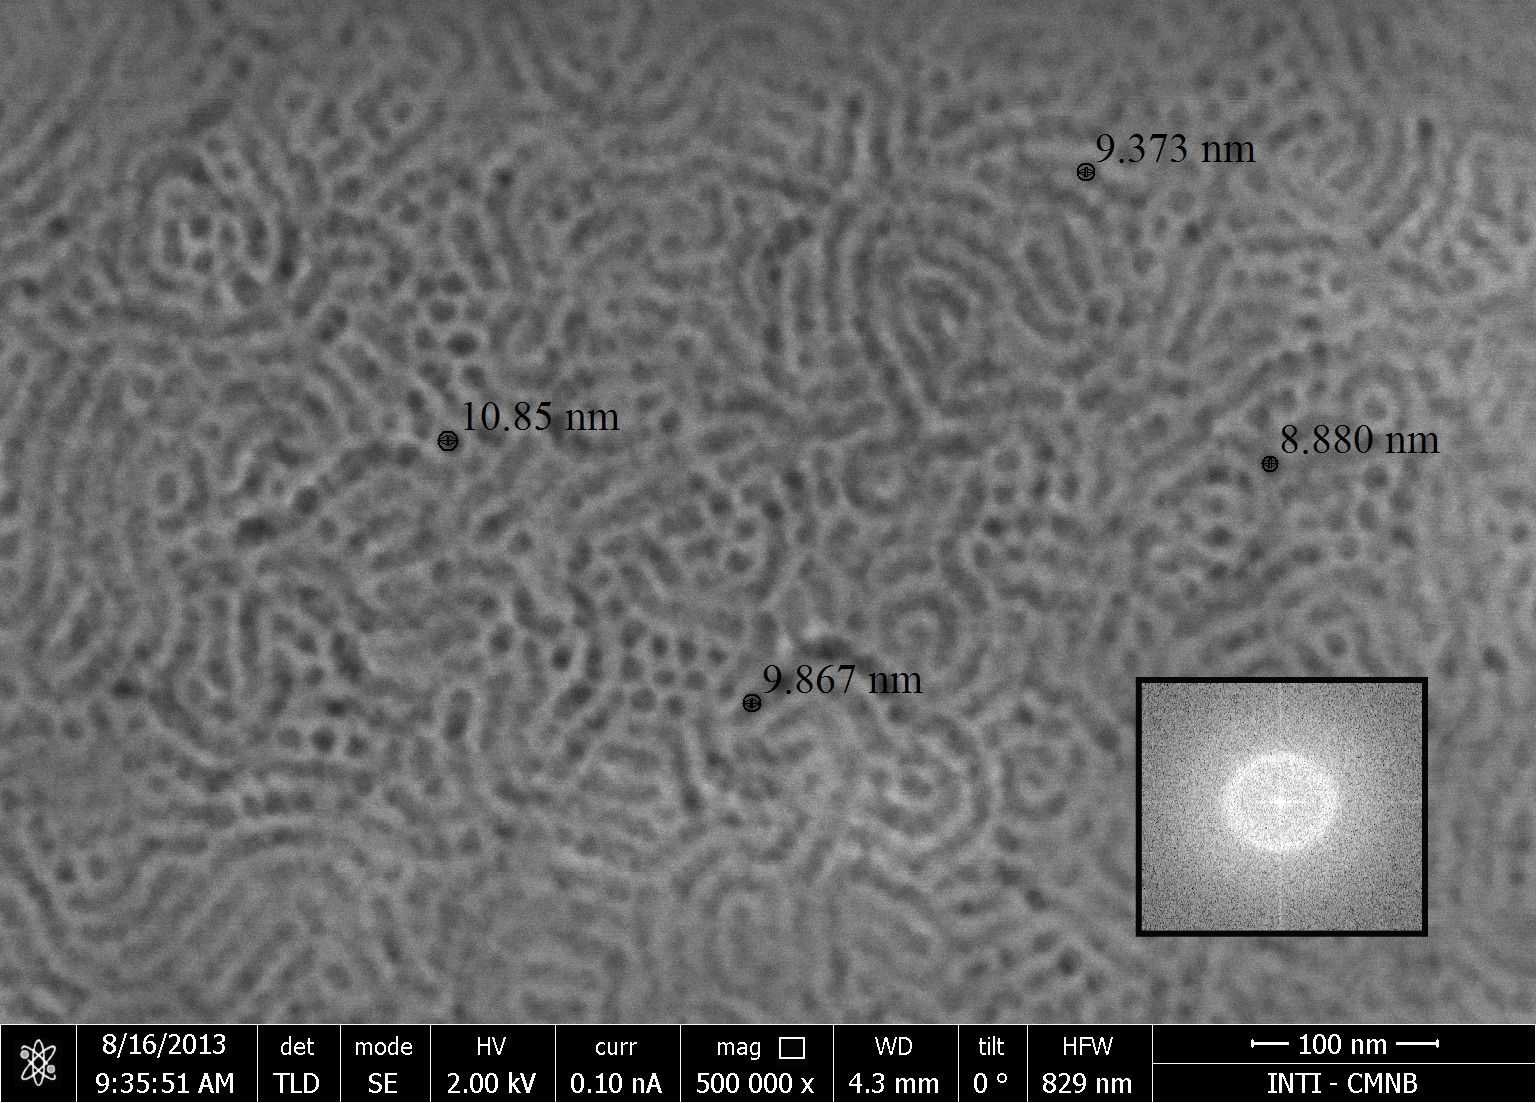
\includegraphics[width=\textwidth]{Imagenes/Superficie-F127-medidas.jpg}
			       		\caption{Microscopía electrón\index{electrón}ica donde se observa la superficie\index{superficie} de una \pdmF\space con poros de \SI{10}{nm} de diámetro en promedio.}
			       		\label{fig:sem_homogeneidad1}
			       		\end{subfigure}
					\begin{subfigure}[t]{0.49\textwidth}
			 	   	    \includegraphics[width=\textwidth]{Imagenes/Perfil-F127-modificado2.jpg}
			       		\caption{Corte transversal por FIB\index{FIB} de una \pdmF\space desde se puede medir el espesor\index{espesor} y ver los nanoporos a lo largo del eje transversal a la película.}
			       		\label{fig:sem_homogeneidad2}
			       		\end{subfigure}
			       	\begin{subfigure}[t]{0.49\textwidth}
			        	\includegraphics[width=\textwidth]{Imagenes/Superficie-CTAB-medidas.jpg}
			       		\caption{Microscopía electrón\index{electrón}ica donde se observa la superficie\index{superficie} de una \pdmC\space con poros de \SI{3}{nm} de diámetro en promedio.}
			       		\label{fig:sem_homogeneidad3}
			       		\end{subfigure}
					\begin{subfigure}[t]{0.49\textwidth}
			 	   	    \includegraphics[width=\textwidth]{Imagenes/Perfil-CTAB.jpg}
			       		\caption{Corte transversal por FIB\index{FIB} de una \pdmC\space desde se puede medir el espesor\index{espesor} de la película. Los nanoporos no se llegan a observar por ser de tamaño muy pequeño para la técnica utilizada.}
			       		\label{fig:sem_homogeneidad4}
			       		\end{subfigure}	
					 \caption[MEB \pdmC\space y \pdmF.]{Microscopia para sistemas de sílice porosos con CTAB y F127 calcinados sobre silicio\index{silicio} con electrodos de Cr\index{cromo}\textbar Au\index{oro} (a y c). Secciones transversales donde se puede apreciar la homogeneidad en el espesor\index{espesor} de las películas (b y d).}
					 \label{fig:sem_homogeneidad}	
				     \vspace*{0.2cm}
				     \end{figure}

		El control del espesor\index{espesor} se logra variando las condiciones de aceleración y velocidad final del \textit{spin-coater}, por lo tanto, para cada condición, se obtiene un espesor\index{espesor} diferente. Las rampas que se han utilizado se muestran en la figura \ref{fig:spin}. El espesor\index{espesor} de las \pdm\space se midió indistintamente por elipsoporosimetría\index{elipsoporosimetría ambiental} ambiental (EPA) o por microscopia\index{microscopía} (FIB/SEM), se puede consultar los detalles de las técnicas en las correspondientes secciones del capítulo \ref{chap:Materiales}. En el gráfico de la figura \ref{fig:esp} se muestra la curva de espesor\index{espesor}es que corresponde a un sistema nanoporoso de SiO$_2$ utilizando F127 como surfactante\index{surfactante}. 

		Según algunos autores, el tratamiento teórico para el deposito de películas poliméricas por \textit{spin-coating}\index{spin@\textit{spin-coating}} revela una dependencia del espesor\index{espesor} con la velocidad según \cite{Norrman2005,Meyerhofer1978,Bornside1989,Lora1990}:
			\begin{equation}
			  t = k_1 \omega^{\alpha}
			  \label{eq:spin_meso}
			  \end{equation}		
		donde $k_1$ y $\alpha$ son constantes empíricas que dependen de la concentración del monómero, del solvente, del sustrato, de la interacción sol/sustrato y  de las propiedades reológicas del sol. Tal como se mostró en la ecuación \ref{eq:spin_meso}, y siguiendo los reportes de la literatura, el valor de $\alpha$ parece mantenerse contante y en las cercanías de $\alpha=-0.5$ para una gran cantidad de polímeros. Ajustando los valores del gráfico \ref{fig:esp} se obtienen los valores de $k_1=6413$ y  $\alpha=-0.442$, los cuales siguen la tendencia esperada; disminución del espesor\index{espesor} con el aumento de la velocidad angular\index{velocidad!angular} y decaimiento exponencial con $\alpha \approx -0.5$. \marginpar{Quizás acá debe hacer la curva de calibración de espesor\index{espesor}es para el CTAB, que no la tengo.}
			\begin{figure}[!ht]
						\begin{center}
						\includegraphics[width=0.70\textwidth]{Graficos/Esp_F127.pdf}
						\caption[Espesor en función de la velocidad de rotación\index{velocidad!de rotación}.]{Espesor en función de la velocidad de rotación\index{velocidad!de rotación} para sistemas \pdmF con velocidades angulares comprendidas en 1000 y \SI{4000}{\minute^{-1}.}}
						\label{fig:esp}
						\end{center}
						\end{figure}

	\subsection{Discusión sobre la adherencia\index{adherencia} de las \pdm}	

		 En numerosos trabajos se ha demostrado la producción de películas delgadas mesoporososas de sílice (tanto con F127 como con CTAB) sobre sustratos de vidrio\index{vidrio} o silicio. Sin embargo, en ninguno se menciona la existencia de problemas de adherencia\index{adherencia} al sustrato\index{sustrato} \cite{Angelome2008,Fuertes2010,Violi2015}. Es más, se conoce que luego de ,tratamientos térmicos para condensar y calcinar el surfactante\index{surfactante}, las películas sufren una contracción uniaxial a lo largo del eje normal a la superficie\index{superficie} del sustrato\index{sustrato} debido a la fuerte adherencia\index{adherencia} al sustrato.\cite{Grosso2004,Soler-Illia2012,Chougnet2005} Se sabe desde hace décadas, que los metales nobles no tienen una buena adherencia\index{adherencia} sobre sustratos no-metálicos\cite{Kern1990,Hieber1976}, con lo cual es de esperar que también se experimenten problemas de adherencia\index{adherencia} al querer depositar un sol\index{sol} sobre una película delgada \index{película!delgada}de Au. 

		\subsubsection{Adherencia de \pdm\space sobre electrodos de Au\index{electrodo!de Au}}

			En el caso en los cuales se depositó \pdm\space estructuradas con Pluronic F127\index{Pluronic F127} sobre películas de Au, se observó, en algunos casos, falta de adherencia. Por ejemplo, en el gráfico \ref{fig:adherencia_F127}, se observa se <<despega>> la \pdm\space durante la adsorción\index{adsorción} de \aminorutenio. La forma del voltagrama (tanto los cambios en la intensidad como los corrimientos en el potencial) se discuten en profundidad en el capitulo \ref{chap:Electroquimica}. Por ahora nos basta con decir que se trata de un cambio repentino de un ciclo de medición al siguiente, pasando de la típica respuesta de una \pdm, a la respuesta habitual de un electrodo desnudo de Au. Esta respuesta sugiere que la película no sufrió una disolución lenta y paulatina, sino que se desprendió del sustrato, total o parcialmente, en algún momento de la medición.
			
				\begin{figure}[th]
				 	   	    \begin{center} 
				        	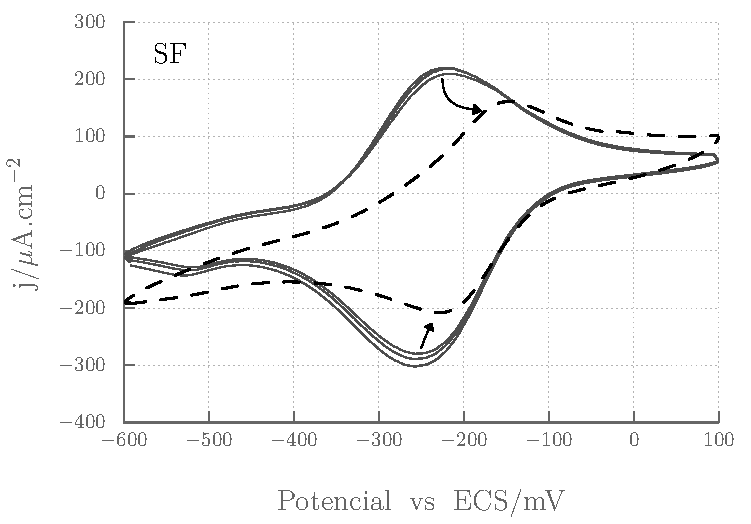
\includegraphics[width=0.70\textwidth]{Graficos/Adherencia_F127.pdf}
				       		\caption[Adherencia de \pdmF \space sobre una película delgada \index{película!delgada}de Au.]{Serie de voltametrías cíclicas consecutivas donde se evidencia la falta de adherencia\index{adherencia} de \pdmF\space sobre electrodo de Au\index{electrodo!de Au}. Las flechas negras indican un cambio repentino de comportamiento. Las VC fueron tomadas a \SI{50}{\milli\volt.\second^{-1}} usando de referencia ESC y con de \ru\space \SI{1}{\milli\Molar}.}
				         	\label{fig:adherencia_F127}
				     		\end{center}
				     		\end{figure}

			En los casos en los cuales se utilizó CTAB como molde para los poros, el comportamiento es algo diferente. Se ven problemas de adherencia\index{adherencia} en la mayoría de los tratamientos alternativos, así como en la calcinación\index{calcinación}. Presentan grietas y fisuras, macro y microscopicas y se observan desprendimientos antes de someter los sensores\index{sensor} a cualquier medición, es decir, apenas terminada la síntesis. Solo se rescataron algunos pocos casos exitosos de formación de \pdmC\space por calcinación\index{calcinación} utilizando como soporte electrodos de Au\index{electrodo!de Au}. Éstos sirvieron para hacer experimentos de EQ conceptuales sobre transporte\index{transporte} en poros (consultar capitulo \ref{chap:Electroquimica}), pero en la generalidad de los casos se observa desprendimiento de la película tal como muestran las imágenes de la figura \ref{fig:CTAB_adherencia}.
	     
				\begin{figure}[th]
		 	   	    \begin{subfigure}[t]{0.49\textwidth}
			        	\includegraphics[width=\textwidth]{Imagenes/Au_FCCTAB_adherencia1.jpg}
			       		\end{subfigure}
					\begin{subfigure}[t]{0.49\textwidth}
			 	   	    \includegraphics[width=\textwidth]{Imagenes/Au_FCCTAB_adherencia2.jpg}
			       		\end{subfigure}
					 \caption[Adherencia de CTAB sobre electrodos.]{Microscopías electrón\index{electrón}icas donde se muestra la falta de adherencia\index{adherencia} de \pdmC\space sobre una película delgada \index{película!delgada}de Au. Obsérvese los círculos grises que corresponden, en realidad a burbujas separadas del sustrato. La imagen de la derecha muestra una porción de \pdmC\space despegada y elevada.}
					 \label{fig:CTAB_adherencia}	
				     \end{figure}
			
			Además de la ya mencionada falta de adherencia\index{adherencia} de los óxidos sobre películas de Au, este desprendimiento se debe, sobre todo, a la interacción CTAB-Au. Es numerosa la información que se encuentra en la literatura sobre la interacción superficial de CTAB sobre películas delgadas y/o nanopartículas de Au. La principal aplicación se basa en la adsorción\index{adsorción} y autoensamblado del CTAB para controlar el crecimiento y estabilización de nanopartículas de Au. \cite{Cheng2003,Smith2008,Lim2014,Meena2013,Wang2013,Hamon2009}

			Cuando el surfactante\index{surfactante} se encuentra en una concentración más alta que la concentración micelar crítica\index{concentración micelar crítica} (cmc), las micelas formadas se adsorben sobre el Au. Su distribución y densidad a largo de la superficie\index{superficie} del electrodo parece depender de la concentración, la orientación cristalina del Au, el solvente y la rugosidad\index{rugosidad} de la superficie\index{superficie}\cite{Meena2013,Lim2014}. La adsorción\index{adsorción} de estas micelas en la superficie\index{superficie} del electrodo, sumada a la poca adherencia\index{adherencia} del propia del SiO$_2$, son los factores que impiden la formación y adherencia\index{adherencia} de \pdmC\space sobre electrodos de Au\index{electrodo!de Au}.
									
		\subsubsection{Modificaciones superficiales}\label{sec:adherencia}

			La adherencia\index{adherencia} de las \pdm\space es crítica para la elaboración de los sensores, y, en función de los resultados expuestos en la sección anterior, es un problema a tener en cuenta durante la fabricación de sensores\index{sensor} electroquímico\index{electroquimico}s\index{electroquimico} basados en electrodos de Au\index{electrodo!de Au}.

			Las estrategias usadas para solucionar estos problemas se basaron en dos conceptos:
				\begin{enumerate}

					\item En la modificación superficial de los electrodos, creando puntos de anclaje al esqueleto inorgánico.

					\item Minimizando el área de contacto electrodo-mesoporoso.

					\end{enumerate}
			La modificación superficial de los electrodos se llevó acabo siguiendo el procedimiento detallado en el capitulo \ref{chap:Materiales}, sección \ref{sec:silanizacion}. Se buscó una molécula\index{moléculas} compatible con el sistema utilizado, que pueda vincular la superficie\index{superficie} del electrodo e integrarse en el esqueleto de las \pdm. Se usó para este fin el 3-mercaptopropil trimetoxisilano\index{mercaptopropil@3-mercaptopropil trimetoxisilano} (MPTMS), el cual es fácilmente de ligar covalentemente al Au\index{oro} por el tiol\cite{Gosser}, y por el otro tiene el silano el cual es perfectamente compatible con el precursor\index{precursor} utilizado\cite{Wu2014,Wu2013,Chen2011}. En la figura \ref{fig:mod_sup} se muestra la molécula\index{moléculas} en cuestión y un esquema de como queda anclado la \pdm\space, mediante el MPTMS, al electrodo.
			
					\begin{figure}[!ht]
							\begin{center}
							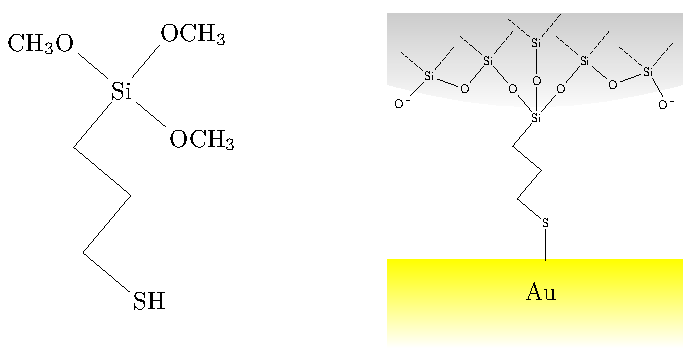
\includegraphics[width=0.60\textwidth]{Esquemas/mod_sup.pdf}
							\caption[Modificación superficial de los electrodos.]{Izquierda: Molécula de  3-mercaptopropil trimetoxisilano\index{mercaptopropil@3-mercaptopropil trimetoxisilano} utilizada como ligante entre los electrodos y las \pdm. Derecha: Esquema pictórico de la modificación superficial con MPTMS.}
							\label{fig:mod_sup}
							\end{center}
							\end{figure}
			
			Una vez realizada la modificación superficial, se llevaron a cabo mediciones EQ, con el objetivo de comparar electrodos modificados y sin modificar, de forma de evaluar el posible bloqueo de los electrodos. La figura \ref{fig:comparaciones_MPTMS} muestra los voltagramas los resultados de dichas comparaciones. Se comparan allí, electrodos con MPTMS y sin MPTMS, recubiertas con \pdm\space y sin recubrir. De estos gráficos comparativos se desprende que el rendimiento electroquímico\index{electroquimico} no se ve afectado significativamente.
	 		
		 			\begin{figure}[th]
			 	   	    \begin{subfigure}[t]{0.49\textwidth}
				        	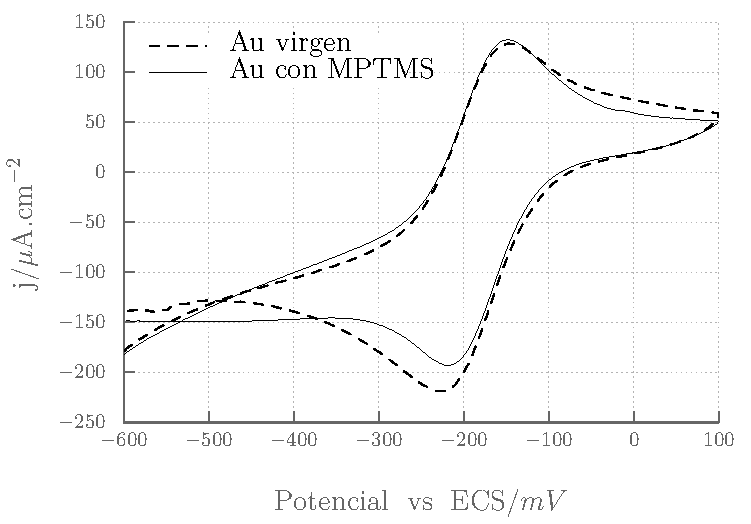
\includegraphics[width=\textwidth]{Graficos/Comparacion_Au-MPTMS.pdf}
				       		\caption{Respuesta EQ de un electrodo desnudo de Au\index{oro} comparado con uno modificado con MPTMS.}	
				       		\end{subfigure}
						\begin{subfigure}[t]{0.49\textwidth}
				 	   	    \includegraphics[width=\textwidth]{Graficos/Comparacion_F127-MPTMS.pdf}
				       		\caption{Respuesta EQ de un electrodo de Au\index{electrodo!de Au}\index{oro} tratados con MPTMS y sin tratar, recubierto con \pdmF\space sobre electrodo de Au\index{electrodo!de Au}.}
				       		\end{subfigure}
						 	\caption[Comparación de superficie\index{superficie}s con y sin MPTMS.]{Voltametrías cíclicas para \aminorutenio\space \SI{1}{\milli\Molar} realizados a \SI{50}{\milli\volt.\second^{-1}} comparando los resultados de electrodos modificados con MPTMS y sin modificar.}
						 \label{fig:comparaciones_MPTMS}	
					     \end{figure}
			
			La segunda estrategía utlizada para promover una mayor adherencia\index{adherencia} de las \pdm\space a los sensores, se basa en minimizar el área de contacto electrodo-mesoporoso. Las mayoría de los resultados discutidos en este capítulo fueron realizados en \pdm\space sobre electrodos plenos de Au. Sin embargo, los sensores\index{sensor} son un conjunto de electrodos o microelectrodo\index{electrodo!microelectrodo}s sobre un sustrato\index{sustrato} dieléctrico (p. ej. SiO$_2$ o vidrio). Eligiendo un diseño adecuado se puede minimizar el área de los electrodos respecto del soporte. De ésta forma las \pdm\space quedan adheridas fuertemente a los sectores donde no está el Au. El resultado final es una película bien adherida sobre una superficie\index{superficie} mixta soporte/electrodos.  La figura \ref{fig:adherencia_microelectrodo} representa de manera esquemática esta situación.
			
				\begin{figure}[!ht]
					\begin{center}
					\includegraphics[width=0.70\textwidth]{Esquemas/adherencia_microelectrodo.pdf}
					\caption[Adherencia a los microelectrodo\index{electrodo!microelectrodo}s.]{Esquema de un corte transversal de los sensores\index{sensor} donde se observan los microelectrodo\index{electrodo!microelectrodo}s y la \pdm\space depositada sobre ellos. Las flechas indican las zonas de baja y alta adherencia.}
					\label{fig:adherencia_microelectrodo}
					\end{center}
					\end{figure}
			
			Ambas estrategias que promueven la adherencia\index{adherencia} de las \pdm\space son complementarias. Esto quiere decir que se puede optimizar el diseño para minimizar la superficie\index{superficie} de electrodos y, a su vez, se pueden tratar los sectores donde queda el Au\index{oro} expuesto con MPTMS, de manera de generar puntos de vinculación entre el mesoporosos y el electrodo. El tratamiento se realiza luego de depositar el Au\index{oro} y antes de realizar el decapado\index{decapar} de la fotorresina\index{fotorresina} (consultar sección \ref{sec:fotolito}, pág. \pageref{sec:fotolito}).		
			% Por último decir que se van a usar de ahora en adelante estos sistema, reforzar con bibliografia.

\section{Métodos alternativos de síntesis de \pdm}
	
	 En esta sección se da cuenta de los resultados obtenidos en la fabricación y caracterización de \pdm\space por métodos alternativos a la calcinación\index{calcinación}. Como ya se mencionó anteriormente, el desarrollo de estos métodos surgió de necesidades que emergieron durante el proceso de fabricación de los sensores. Minimizar la diferencia de expansión térmica entre las películas delgadas mesoporosas y metálicas, evitar procesos difusivos, ampliar sustancialmente la gama de sustratos y, mejorar la adherencia\index{adherencia} y disminuir costos, entre otros

	 En este sentido, se idearon procesos que permitan bajar la temperatura (hasta \SI{130}{\celsius}) sin perder grado de condensación\index{condensación} y manteniendo las características espaciales de los poros. Al\index{aluminio} no calcinar, se agrega una etapa extra, la eliminación\index{eliminación} del surfactante\index{surfactante}. Presentamos a continuación una tabla con la nomenclatura y una breve reseña de los procesos que se exploró.

	 	 \begin{table}[ht!] 
		 	 \caption[Tratamientos alternativos de síntesis de \pdm]{Nomenclatura de los métodos alternativos de síntesis de \pdm.}
			 \begin{tabular}{>{\raggedright\arraybackslash}m{1.9cm}>{\centering\arraybackslash}m{1cm}>{\raggedright\arraybackslash}m{0.9cm}>{\raggedright\arraybackslash}m{6.62cm}} 
			 \toprule
				 Método   &  Nomenclatura$^*$&  & Descripción \\ \midrule
				 Calcinado & CalSC CalSF& &  Condensación\index{condensación} \SI{130}{\celsius} \SI{1}{hora}\hspace{2cm} Extracción \SI{350}{\celsius} \SI{2}{hora}\hspace{2cm} \\ \midrule
				 Simplifciado & SimSC SimSF& &  Condensación\index{condensación} \SI{130}{\celsius} \SI{1}{hora}\hspace{2cm} Extracción IpOH / H$_2$O pH\index{pH}=2 \\ \midrule
				 Prolongado & ProSC ProSF& & Condensación\index{condensación} \SI{130}{\celsius} \SI{7}{dias}\hspace{2cm} Extracción IpOH / H$_2$O pH\index{pH}=2 \\ \midrule				
				 Vacío & VacSC VacSF VacZSF& &  Condensación\index{condensación} \SI{130}{\celsius} \SI{7}{dias}, P=\SI{e-5}{\milli\bar}\hspace{2cm} Extracción IpOH / H$_2$O pH\index{pH}=2 \\ \midrule
				 Ácido & ÁciSC ÁciSF& &  Condensación\index{condensación} en atmósfera de HCl\index{acido@ácido!clohídrico}\hspace{2cm} Extracción IpOH / H$_2$O pH\index{pH}=2 \\ \midrule
				 Al\index{aluminio}calino & Al\index{aluminio}cSC Al\index{aluminio}cSF& & Condensación\index{condensación} en atmósfera de NH\index{amoniaco}$_3$\hspace{2cm} Extracción IpOH / H$_2$O pH\index{pH}=2 \\ 
				\bottomrule
				   \end{tabular}\vspace*{2pt}
		    	  	\footnotesize{$^*$SC=sílice/CTAB, SF=sílice/F127, ZSF=circonio-sílice/F127}
				   	\label{tabla:tratamientos}
				   \end{table}
				   \vspace*{-0.22cm}

	 Se exponen primero los resultados de las caracterizaciones de las \pdm\space obtenidas por calcinación\index{calcinación}. El propósito de ésto es tener datos de referencia para comparar con los métodos alternativos. Luego se discuten los resultados que se obtuvieron por cada uno de ellos y se resumen en la tabla \ref{tabla:resultados}. Finalmente, se hace una discusión global comparando cada una de las técnicas, para cada uno de los métodos. Para facilitar la lectura, la mayoría de los gráficos, microscopia\index{microscopía}s y espectros de la sección se encuentran en el anexo C.

	\subsection{Método por calcinación\index{calcinación}}
	 	
	 		El tratamientos por calcinación\index{calcinación} luego del depósito\index{depósito} del sol\index{sol} es una ruta sintética clásica utilizada por muchos autores para la producción de películas delgadas mesoporosas de óxidos\cite{Soler-Illia2002a,Brinker1999,Soler-Illia2006,Grosso2004,Innocenzi2013,angelome2011}. Consiste en estabilizar las \pdm\space en humedad, temperatura y luego calcinar a \SI{350}{\celsius} para calcinar el molde. Los detalles técnicos se pueden consultar en la sección \ref{sec:cond_y_extr}, pág. \pageref{sec:cond_y_extr}.

	 	\subsubsection{Análisis de la porosidad}

		 Como veremos mas adelante la porosidad\index{porosidad} y accesibilidad\index{accesibilidad} nos determinarán la cantidad de analito que se adsorbe o pasa a través de las \pdm, por este motivo es fundamental poder cuantificar dichas características. 

		 Del estudio de las películas por MEB se puede obtener información muy valiosa como tamaño y distribución de los poros\index{distribución!de poro}, así como estudios de la organización espacial de los mismos. En la figura \ref{fig:F127_Si_Au} se muestran imágenes de MEB para películas \pdmF. De éstas, se hace obtiene que se trata de un arreglo de poros con orden local, con tamaños próximos a los de \SI{10}{\nm} de diámetro, coincidiendo la con información existente en la literatura\cite{urade2005,angelome2011,lee2006}.  

			\begin{figure}[th]
		 	   	    \begin{subfigure}[t]{0.49\textwidth}
			        	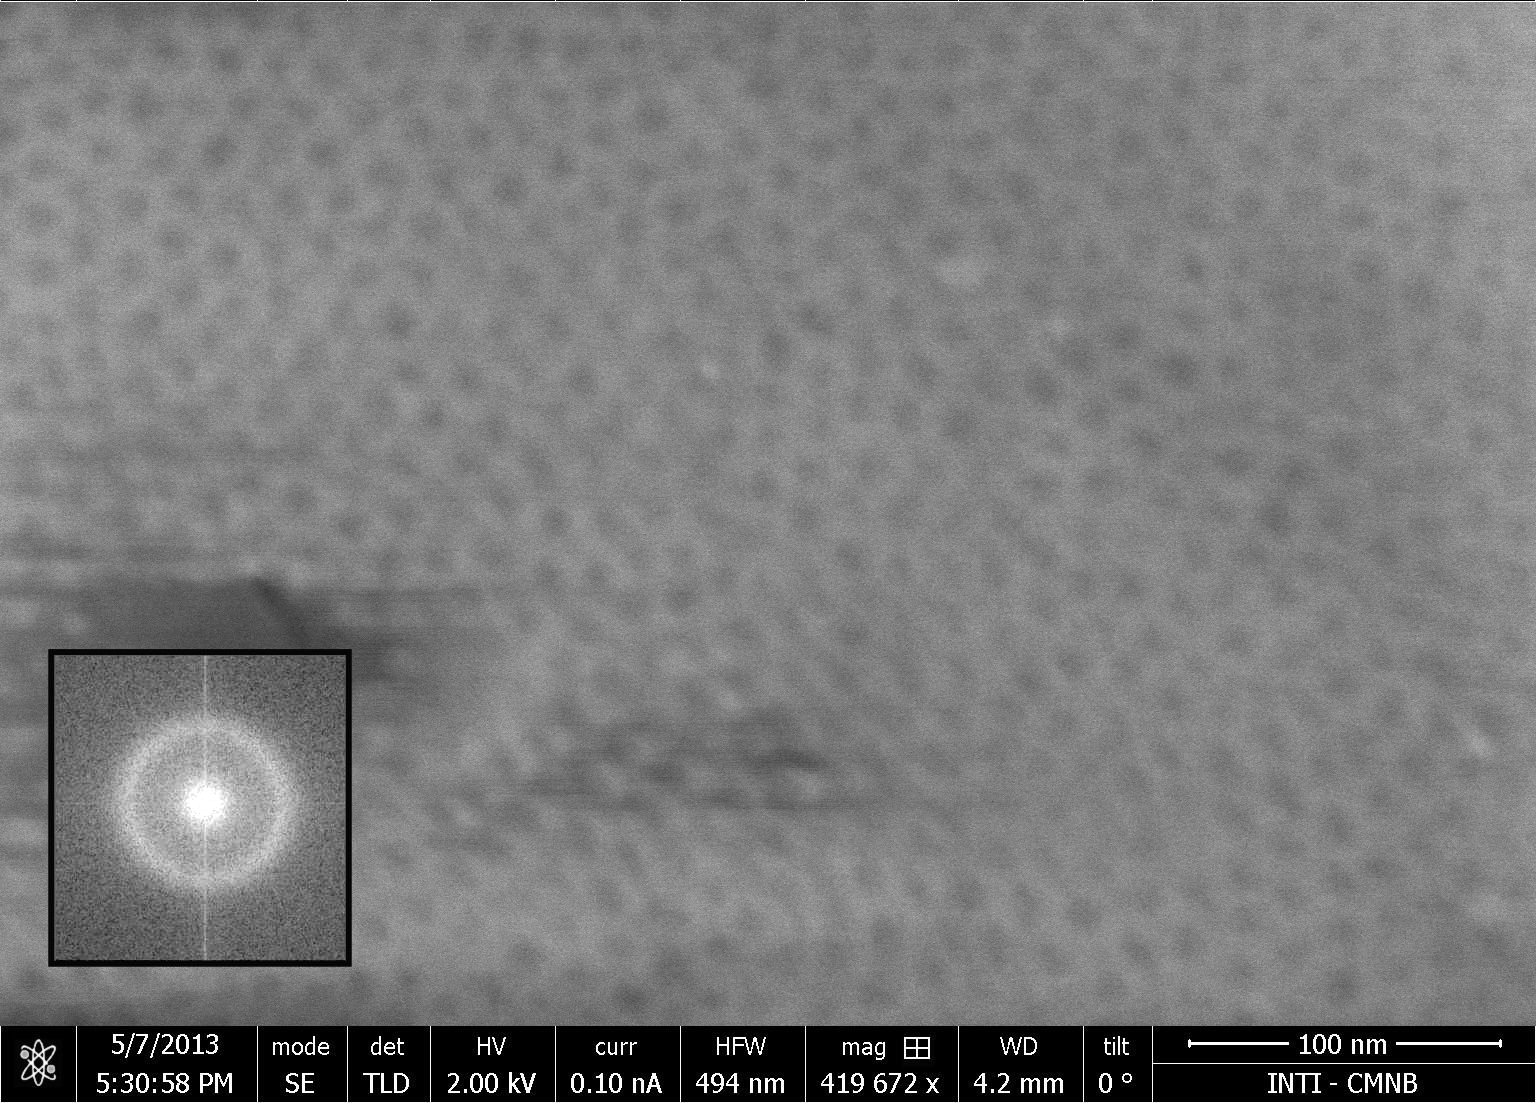
\includegraphics[width=\textwidth]{Imagenes/F127_Si_sup.jpg}
			       		\end{subfigure}
					\begin{subfigure}[t]{0.49\textwidth}
			 	   	    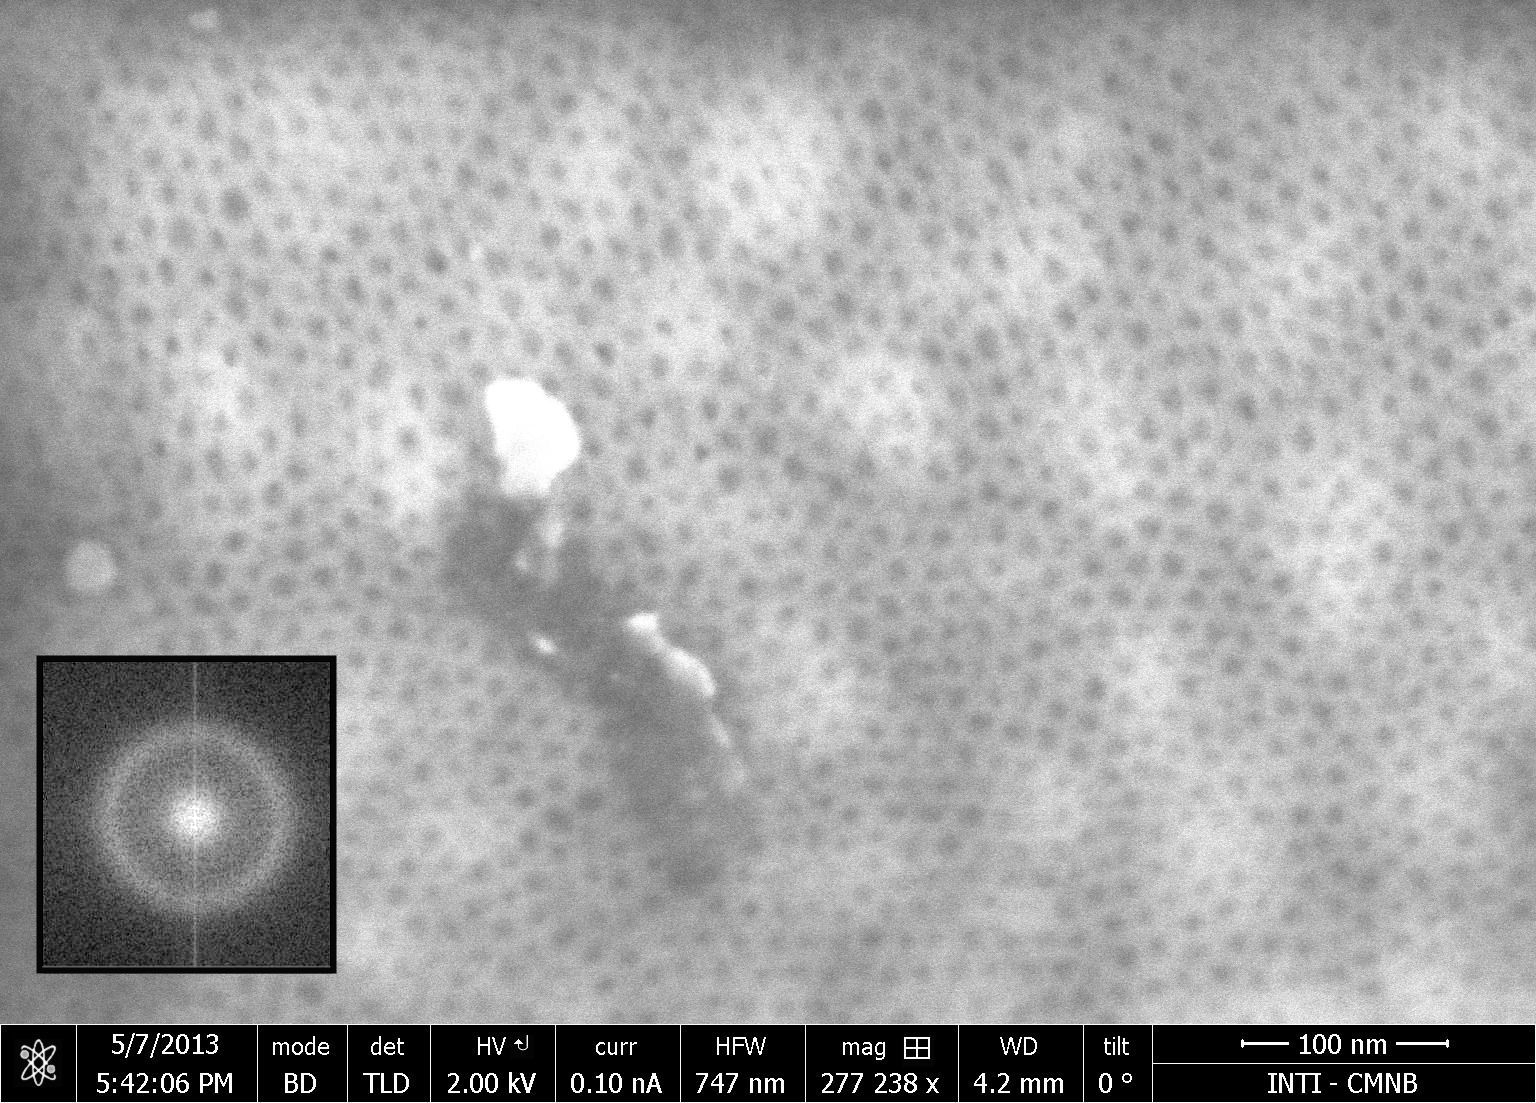
\includegraphics[width=\textwidth]{Imagenes/F127_Au_sup.jpg}
			       		\end{subfigure}
					\caption[MEB arreglo poroso sobre Si y Au.]{Microscopía electrón\index{electrón}ica de barrido de \pdmF\space donde se observa la distribución y homogeneidad de los poros en superficie\index{superficie}. Izquierda: sobre sustrato\index{sustrato} de silicio. Derecha: sobre sustrato\index{sustrato} de Au.}	 
					 \label{fig:F127_Si_Au}
					 \end{figure}

		 En el caso de las películas porosas estructuras con CTAB es más difícil hacer una análisis por MEB, ya que el diámetro de los poros ($\approx$ \SI{3}{\nm}) esta en el límite de resolución la técnica. Sin embargo, alcanza para  ver que existe un sistema de poros (ver figura \ref{fig:sem_homogeneidad3}). En este caso, para hacer un estudio por imágenes mas completo, se debería recurrir a microscopia\index{microscopía} electrón\index{electrón}ica de transmisión (MET).

		 El estudio por MEB es sumamente útil en muchos aspectos; sin embargo, la información que brinda es de áreas muy pequeñas, superficial y no da información completa sobre la conectividad\index{conectividad} y cuello\index{cuello de poro}s de las películas. Es por ello recurrió a la técnica de elipsoporosimetría\index{elipsoporosimetría ambiental} ambiental (EPA). Es una técnica promedio donde podemos obtener información valiosa sobre la accesibilidad\index{accesibilidad} del agua a los poros, volumen poroso de las \pdm, distribución de tamaños de poros y cuello\index{cuello de poro}s y variación del espesor\index{espesor} en función de la presión de vapor\index{presión de vapor} de agua relativa a la presión de saturación ($\text{P/P}_s$). Para valores crecientes de P/P$_s$, la adsorción\index{adsorción} en los mesoporos se produce a través de la formación de una monocapa\index{monocapa} y luego de multicapas de moléculas de agua sobre las paredes de los poros, seguida de condensación\index{condensación} capilar, es decir, llenado de los poros con agua líquida. La posterior disminución de la presión externa resulta en la desorción\index{desorción} mediante evaporación capilar, vaciando el centro de los poros, seguida por la desorción\index{desorción} de la multicapa de solvente de las paredes de los poros. Para cada punto de P/P$_s$ en equilibrio se tiene un valor del índice de refacción efectivo ($n$), de esta forma se construye la isoterma\index{isoterma} de adsorción\index{adsorción}/desorción de agua. Los cálculos realizados para obtener información estructural (volumen poroso, y distribución de poro\index{poro} y cuello\index{cuello de poro}) a partir de las isoterma\index{isoterma}s se basaron en el protocolo detallado los trabajos del grupo deSánchez\index{Sánchez} y Baklanova\index{Baklanova}\cite{Baklanov2000,Boissiere2005,Sakatani2006}. Los detalles experimentales de esta técnica se presentaron en el capitulo \ref{sec:elipso}, pág. \pageref{sec:elipso}.

		 En las figuras \ref{fig:F127_EPA} y \ref{fig:CTAB_EPA} se presentan las isoterma\index{isoterma}s de adsorción\index{adsorción} de agua para sistemas calcinados \pdmF\space y \pdmC. Se observa que ambas son de tipo IV, según la clasificación de Brunauer\index{Brunauer}\cite{Gregg1967,Violi2015,Fuertes2010}. Este tipo de isoterma\index{isoterma}s con histéresis\index{histéresis} entre la rama de adsorción\index{adsorción} y la de desorción\index{desorción} es característica de materiales con mesoporos, donde los poros se llenan por condensación\index{condensación} capilar. Por otro lado el ciclo de histéresis\index{histéresis} es de tipo H1, según la clasificación IUPAC\index{IUPAC}, lo cual indica poros de tamaño uniforme.\cite{Gregg1967,Lowell2004,Sing1985}

		 En las figuras \ref{fig:F127_PSD} y \ref{fig:CTAB_PSD} se muestran se muestran las distribuciones de tamaño de poro\index{poro} para estos sistemas. Estas distribuciones se obtuvieron a partir de las isoterma\index{isoterma}s, y se extrajo información estructural tanto de la rama de adsorción\index{adsorción} como de la de desorción\index{desorción}.


		     	  	\begin{figure}[!ht]
		     	  		\begin{subfigure}[t]{0.495\textwidth}
		     	  		\includegraphics[width=\textwidth]{Graficos/SI_F127_Calcinado_EPA.pdf}
						\caption{Elipsoporsimetría de una \pdmF\space depositada sobre silicio\index{silicio} sintetizada por calcinación\index{calcinación}.}
						\label{fig:F127_EPA}
						\end{subfigure}
						\begin{subfigure}[t]{0.495\textwidth}
		     	  		\includegraphics[width=\textwidth]{Graficos/SI_F127_Calcinado_PSD.pdf}
						\caption{Distribución de tamaño de poro\index{poro} y cuello\index{cuello de poro} correspondientes a la isoterma\index{isoterma} de (a).}
						\label{fig:F127_PSD}
						\end{subfigure}
						\caption[Elipsoporosimetría para sistemas \pdmF.]{Curva de adsorción\index{adsorción}/desorción de agua para una \pdmF\space (a). La misma corresponde a una isoterma\index{isoterma} de tipo IV con un lazo de histéresis\index{histéresis} de tipo H1, lo cual se concuerda con materiales mesoporosos con tamaño de poros uniformes. Distribución de poros y cuello\index{cuello de poro}s (b) con tamaño de poros uniformes, de aproximadamente \SI{10}{\nm} de diámetro.}
						\end{figure}
					\begin{figure}[!ht]
		     	  		\begin{subfigure}[t]{0.495\textwidth}
		     	  		\includegraphics[width=\textwidth]{Graficos/SI_CTAB_Calcinado_EPA.pdf}
						\caption{Elipsoporsimetría de una \pdmF\space sobre sustrato\index{sustrato} de silicio\index{silicio} sintetizada por el método clásico de calcinación\index{calcinación}.}
						\label{fig:CTAB_EPA}
						\end{subfigure}
						\begin{subfigure}[t]{0.495\textwidth}
		     	  		\includegraphics[width=\textwidth]{Graficos/SI_CTAB_Calcinado_PSD.pdf}
						\caption{Distribución de tamaño de poro\index{poro} y cuello\index{cuello de poro} correspondientes a la isoterma\index{isoterma} de (a).}
						\label{fig:CTAB_PSD}
						\end{subfigure}
						\caption[Elipsoporosimetría para sistemas \pdmC.]{Curva de adsorción\index{adsorción}/desorción de agua para una \pdmC\space (a). La misma corresponde a una isoterma\index{isoterma} de tipo IV con un lazo de histéresis\index{histéresis} de tipo H1, lo cual se concuerda con materiales mesoporosos con tamaño de poros uniformes. Distribución de poros y cuello\index{cuello de poro}s (b) con tamaño de poros uniformes, de aproximadamente \SI{3}{\nm}.}
						\end{figure}	
		
		 	Del conjunto de resultados presentados se puede resaltar que son películas homogéneas, sin grietas microscopicas, con poroso de orden local y distribución. Las \pdm\space estructuras con F127 presentan poros	y cuello\index{cuello de poro}s de 9 y \SI{4.5}{\nm} de diámetro respectivamente, mientras qeu las estrcuturas con CTAB 2.5 y \SI{2}{\nm}. También se pueden extraer los valores de $n$, porcentaje de volumen poroso (\%V) y espesor\index{espesor} los cuales se resumen en la tabla \ref{tabla:resultados}. Estos valores son los que se usarán para establecer un parámetros de condensación\index{condensación} y porosidad\index{porosidad} de las \pdm y se usaran como semilla para la discusión comparativa con los resultados obtenidos para el resto de los tratamientos.

	    \subsubsection{Análisis por FTIR}\label{sec:Analisis_IR}

		 Son muchos los trabajos en los cuales caracterizan las películas delgadas de SiO$_2$ por IR\cite{Olsen1989,Almeida1990,Redol1997,Innocenzi2003}, y también muchos que otros que hacen usos de estos resultados \cite{Angelome2008,Calvo2008,Calvo20210}.
		 El análisis de espectroscopia\index{espectroscopia} infrarroja por transformada de Fourier (FTIR) se utilizó en esta tesis para identificar y caracterizar la estructura inorgánica porosa de SiO$_2$, evaluar comparativamente condensación\index{condensación} del óxido, y determinar la presencia de grupos orgánicos, entre ellos residuos de surfactante\index{surfactante}. El seguimiento por FTIR\index{FTIR} de la presencia de surfactante\index{surfactante} es muy importante sobre todo en aquellos tratamientos donde las películas no fueron sometidas a calcinación\index{calcinación}.

		Innocenzi\index{Innocenzi} ha realizado un análisis completo y bien fundamentado sobre las vibraciones\index{vibración} en el IR, de películas delgadas de SiO$_2$ tanto densas como porososas.\cite{Innocenzi2003} Para los enlaces Si-O-Si, se observa la presencia de 4 modos de vibración\index{vibración} óptico-trasversales (TO$_x$) y 4 modos óptico-longitudinales (LO$_x$) para películas delgadas de SiO$_2$. En experimentos de incidencia normal a la superficie\index{superficie}, solo deberían excitarse las vibraciones\index{vibración} óptico-transversales, sin embargo se observan banda de vibraciones\index{vibración} correspondientes a modos óptico-longitudinales asociadas a oscilaciones colectivas acopladas TO-LO.\cite{Pai1986,Grosse1986,Innocenzi2003}

		 	 \begin{figure}[!ht]
						\begin{center}
						\includegraphics[width=0.85\textwidth]{Graficos/IR_Denso.pdf}
						\caption[FTIR SiO$_2$ denso y SiO$_2$ mesoporoso.]{Espectro de absorción de IR de una película SiO$_2$ denso depositada por \textit{sputtering }comparada con una de SiO$_2$ mesoporoso. Se observa, para las \pdm, la aparición de un marcado hombro en \SI{1180}{\per\cm} debido al acoplamiento TO$_3$-LO$_3$ y un pico correspondiente a la vibración\index{vibración} $\nu$Si-OH.}\index{sputtering@\textit{sputtering}}
						\label{fig:IR-denso}
						\end{center}
						\end{figure}

		 El modo TO$_1$, presenta una banda débil $\approx$\SI{460}{\cm^{-1}} asociada a movimientos de balanceo; el modo TO$_2$ está asociado a un estiramiento simétrico con un pico débil cercano a $\approx$\SI{800}{\cm^{-1}}; y el modo TO$_3$, el cual presenta un pico intenso centrado en $\approx$\SI{1075}{\cm^{-1}}, se encuentra asociado a las vibraciones\index{vibración} asimétricas del enlace Si-O-Si. Respecto de los modos ópticos-longitudinales, LO$_1$ y LO$_2$ no son visibles, y LO$_3$, aparece como un hombro de la banda TO$_3$ a mayores frecuencias. La observación experimental de los modos TO$_4$ y LO$_4$ es escasa, cuando se observa aparecen como bandas débiles en la zona comprendida entre 1200 y \SI{1150}{\cm^{-1}} \cite{Pai1986,Grosse1986}.
				 	
		 Otra observación relevante, realizadas por Al\index{aluminio}meida y Pantano\cite{Almeida1990}, es la naturaleza del hombro presente en $\approx$\SI{1180}{\cm^{-1}}, el cual se intensifica con el aumento de la porosidad\index{porosidad} de la película y lo asocia a un acoplamiento de los modos LO$_3$ y TO$_3$ con predominancia de carácter LO. Este fenómeno parece estar asociado a la dispersión de la radiación\index{radiación} IR dentro de los poros y la consecuente activación del modo longitudinal.	
			
		 Se pudo corroborar dicha observación en los espectros de la figura \ref{fig:IR-denso}, donde se compara una \pdm\space con una película delgada \index{película!delgada}de SiO$_2$ depositada por \textit{sputtering}\index{sputtering@\textit{sputtering}}.  Al\index{aluminio}lí se ve el hombro bien acentuado para la \pdm\space y una banda en $\approx$\SI{965}{\cm^{-1}} asociada al estiramiento Si-OH/Si-O$^-$; mientras que para la película de SiO$_2$ denso se observa la ausencia del hombro, aparición de la incipiente banda de LO$_4$ y desaparece la banda del Si-OH/Si-O$^-$.

		 Además del análisis de la estructura inorgánica, se utilizó FTIR\index{FTIR} para evidenciar la presencia del surfactante\index{surfactante} usado de molde para los poros. Se centrará la atención en las bandas que corresponden a las vibraciones\index{vibración} del enlace C-H, las cuales aparecen en la zona de 2950 a \SI{2850}{\cm^{-1}}. En la figuras \ref{fig:IR_F127_calciando} y \ref{fig:IR_CTAB_calcinado} se comparan \pdm\space calcinadas y sin calcinar para los surfactante\index{surfactante}s utilizados. Se ve como desaparecen las bandas correspondientes a al vibración\index{vibración} C-H debido a la eliminación\index{eliminación} del surfactate. Se conserva la forma del hombro a $\approx$\SI{1180}{\cm^{-1}} indicador de una estructura porosa y se observa la banda en en $\approx$\SI{965}{\cm^{-1}} asociada al estiramiento Si-OH/Si-O$^-$, el cual según algunos autores sólo desaparece cuando las películas son sometidas a T$>$\SI{500}{\celsius}.\cite{Innocenzi2003,Almeida1990,Bertoluzza1982}

				\begin{figure}[!ht]
						\begin{center}
						\includegraphics[width=0.85\textwidth]{Graficos/IR_F127.pdf}
						\caption[FTIR para una \pdmF.]{Espectro de absorción para una \pdmF\space antes y después de calcinar, donde se puede apreciar la aparición de un pico fuerte el cual correspondiente al surfactante\index{surfactante} F127.}
						\label{fig:IR_F127_calciando}
						\end{center}
						\end{figure}
				
				\begin{figure}[!ht]
						\begin{center}
						\includegraphics[width=0.85\textwidth]{Graficos/IR_CTAB.pdf}
						\caption[FTIR para una \pdmC.]{Espectro de absorción para una \pdmC\space antes y después de calcinar, donde se puede apreciar la aparición de un pico fuerte el cual correspondiente al surfactante\index{surfactante} CTAB.}
						\label{fig:IR_CTAB_calcinado}
						\end{center}
						\end{figure}		
		 
		 Estos espectros IR, obtenidos para películas calcinadas, se utilizaran de parámetro para comparar con los IR de \pdm\space producidas por métodos alternativos. Por un lado, se evalúa la presencia de poros, indicado por la presencia del hombro LO$_3$-TO$_3$. Por otro, el grado de condensación\index{condensación}, siguiendo la relación de picos Si-O-Si/Si-OH. Por último, se corrobora la eliminación\index{eliminación} del surfactante\index{surfactante} por ausencia de la banda $\approx$\SI{2900}{\per\cm} correspondiente a la vibración\index{vibración} C-H.

		 En la tabla que sigue, se asignan las vibraciones\index{vibración} observadas que servirán de referencia para el análisis de resultados de las próximas seccciones.

		 	\begin{table}[ht!] 
		 	 \caption[Asignación de vibraciones\index{vibración} en el IR]{Bandas y asignación de vibraciones\index{vibración} en el IR frecuentemente observadas a lo largo de la tesis.}
			 \begin{tabular}{>{\raggedright\arraybackslash}m{2.6cm}>{\centering\arraybackslash}m{2.55cm}>{\raggedright\arraybackslash}m{5.7cm}} 
			 \toprule
				 Posición (\si{\per\cm})   &  Vibración &  Presente en \\ \midrule
				 3500-3000	& $\nu_\text{OH}$ & H$_2$O, 2-propanol\index{propanol@2-propanol} \\ \midrule
				 2950-2850  & $\nu_\text{C-H}$ & Molde (CTAB, Pluronic F127\index{Pluronic F127}) \\ \midrule
				 2450		& CO$_2$ & CO$_2$ ambiental \\ \midrule
				 2000-1200  & H$_2$O & Estructura fina del H$_2$O \\ \midrule
				 1250		& $\nu_\text{Si-O-Si}$ & SiO$_2$ Denso LO$_3$ \\ \midrule
				 1170		& $\nu_\text{Si-O-Si}$ & SiO$_2$ Denso LO$_4$ \\ \midrule
				 1075		& $\nu_\text{Si-O-Si}$ & SiO$_2$ TO$_3$ \\ \midrule
				 1180 (hombro) & $\nu_\text{Si-O-Si}$ & SiO$_2$ poroso acoplamieno LO$_3$-TO$_3$ \\ \midrule
				 965 		& $\nu_\text{Si-OH}$ & SiO$_2$ parcialmente condensado\\ \midrule 
				 800		& $\nu_\text{Si-O-Si}$ & SiO$_2$ TO$_2$ \\
				 \bottomrule
				   \end{tabular}
				   	\label{tabla:ftir}
				   \end{table}

	    \subsubsection{Accesibilidad de las PDM}\label{sec:acc}

			Hasta ahora se han evaluado muchos de los aspectos fundamentales para poder pensar en utilizar las películas mesoporosas de óxido de silicio\index{silicio!oxido de}\index{silicio} como componentes de sensores: estructura porosa, volumen poroso, compatibilidad de sustratos, técnicas de depósito, control del espesor\index{espesor}, etc. 

			Sin embargo, se debe tener en cuenta un aspecto crítico para utilizar estas películas como parte de un sensor\index{sensor} electroquímico\index{electroquimico}. Se tiene que garantizar el libre acceso de los analitos a través de los nanoporos, de forma de poder difundir hasta la superficie\index{superficie} del electrodo, y que tenga lugar allí, la reacción electroquímica\index{electroquimico}.

			Para ello, se coloca una solución con una sonda\index{sonda} electroquímica\index{electroquimico} adecuada, en la celda de medición. La forma en que fueron tomadas las medidas se explica en la sección \ref{sec:medidas_eq}, pág \ref{sec:medidas_eq}. 

			La figura \ref{fig:accesibilidad} muestra dos voltametrías cíclicas, una para \pdmF\space y otra para \pdmC en presencia de \aminorutenio\space \SI{1}{\milli\Molar} en solución de KCl \SI{0.1}{\Molar}. En ambos voltagramas se registra una respuesta electroquímica\index{electroquimico}, demostrando que la superficie\index{superficie} del electrodo se encuentra accesible. Los resultados sugieren que existe un camino percolativo en las \pdm, tanto si se estructuran con F127 o con CTAB, que permite, o bien que la señal electroquímica\index{electroquimico} se propague desde el seno de la solución hasta el electrodo o bien que el analito difunda desde la solución al electrodo. Los fenómenos de trasporte involucrados en este experimento, son tema central de esta tesis y se discuten en detalle en el capitulo \ref{chap:Electroquimica}, así como la forma de los voltagramas. En dicho capítulo se analizan la separación del potencial entre los picos anódico y catódico y las intensidades de los mismos relativa a un electrodo de Au\index{electrodo!de Au}\index{oro} sin recubrir. 

						\begin{figure}[th]
				 	   	    \begin{subfigure}[t]{0.495\textwidth}
				        	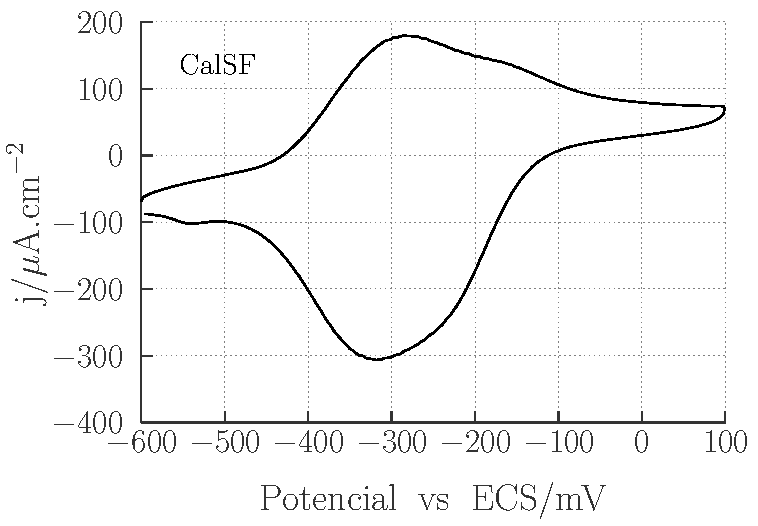
\includegraphics[width=\textwidth]{Graficos/SF-accesibilidad.pdf}
				       		\caption{Voltametría Cíclica sobre \pdmF}
				         	\end{subfigure}
				         	\begin{subfigure}[t]{0.495\textwidth}
				        	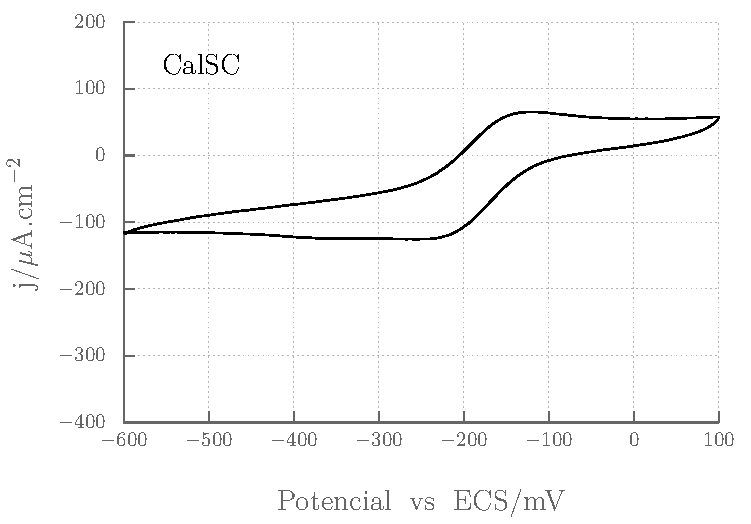
\includegraphics[width=\textwidth]{Graficos/SC-accesibilidad.pdf}
				       		\caption{Voltametría Cíclica sobre \pdmC}
				         	\end{subfigure}
				     		\caption[Accesibilidad electrodo de trabajo\index{electrodo!de trabajo}.]{Voltametrías Cíclicas de \aminorutenio\space \SI{1}{\milli\Molar} sobre Au\index{oro} recubierto con \pdm\space con una velocidad de barrido\index{velocidad!de barrido} \SI{50}{\milli\volt\per\second} usando de referencia ESC.}
				     		\label{fig:accesibilidad}
				     		\end{figure}
	
	 \subsection{Método simplificado}

		 	De todos los tratamientos pos-depósito, el simplifcado, como su palabra lo indica, es el más simple de todos. Consistió en estabilizar las \pdm\space a \SI{130}{\celsius} durante \SI{1}{\hour} y luego extraer el surfactante\index{surfactante} en reflujo\index{reflujo} de 2-pronanol durante \SI{15}{\minute}. 
			
			En el análisis por microscopia\index{microscopía} se aprecia que las \pdmF\space sometidas a éste tratamiento se adhieren bien y quedan bien formadas, sin grietas ni discontinuidades y con poros bien formados sobre la superficie\index{superficie} para ambos sustratos, tanto sobre Au\index{oro} como sobre Si (figura \ref{fig:Microscopia_F127_simplificado}). Las \pdmC\space sobre silicio\index{silicio} también adhieren bien y no presentan grietas, mientras que sobre Au\index{oro} presentan grietas y discontinuidades en su estructura (figura \ref{fig:Microscopia_CTAB_simplificado}), lo cual se adjudica al hecho de la adsorción\index{adsorción} del bromuro sobre el Au, tema que ya fue discutido en la sección \ref{sec:adherencia}, pág. \pageref{sec:adherencia}. 
			
			La caracterización por elipsoporismetría para las \pdmF\space resulto en una isoterma\index{isoterma} tipo IV con histéresis\index{histéresis} H5 para las \pdmC\space y tipo IV con histéresis\index{histéresis} H1 para las \pdmF.\cite{Thommes2015}. Los sistemas estructurados con CTAB presentan una porosidad\index{porosidad} alta, aproximadamente del 40\%, con una histéresis\index{histéresis} pequeña entre las ramas de adsorción\index{adsorción} y desorción\index{desorción} de la isoterma\index{isoterma}. Esto significa, que no hay prácticamente diferencia entre el tamaño de poro\index{poro} y cuello\index{cuello de poro} (figuras \ref{fig:CTAB_simplificado_EPA}  y \ref{fig:CTAB_simplificado_PSD}). Este diámetro de poro\index{poro} pequeño se puede atribuir a que el surfactante\index{surfactante} ha sido sólo parcialmente eliminado de la estructura, estrechando el tamaño de poro\index{poro} hasta hacerlo prácticamente igual tamaño de los cuello\index{cuello de poro}s.
			En el caso de los sistemas \pdmF\space la adsorcion de agua se produce en una única etapa mientras que la desorción\index{desorción} ocurren a dos valores de presión diferentes, a P/P$_s=0,65$ y a P/P$_s=0,45$ (figura \ref{fig:F127_simplificado_EPA_2}). 

			Thielemann \cite{Thielemann2011} y Groen\index{Groen}\cite{Groen2003} proponen que este comportamiento se produce al desorber el agua ocluida en poros, que están más o menos <<bloqueados>> por el diámetro de los cuello\index{cuello de poro}s, tal como se ejemplefica en la figura \ref{fig:thielemann}. Al\index{aluminio} producirse la desorción\index{desorción} del agua a través de cuello\index{cuello de poro}s de distinto tamaño, la fuerza  necesaria para vencer la tensión superficial\index{tensión superficial} debe ser mayor, desorbiendo a menor P/P$_s$ cuanto menor sea el diámetro de los cuello\index{cuello de poro}s; tal como predice la ecuación de Kelvin\index{Kelvin} (ver ecuación {\ref{eq:kelvin}). Esta observación se repite para varios de los tratamientos practicados e indica una población de cuello\index{cuello de poro}s con una doble distribución\index{distribución!doble} de tamaño (figura \ref{fig:F127_simplificado_PSD}). Esto sugiere dos posibilidades, la existencia de dos sistemas porosos no conectados entre sí, ó falta de condensación\index{condensación} en el sistema porosos con cuello\index{cuello de poro}s o poros medianamente ocluidos por sílice parcialmente condensada.

			%Grafico de Thielemann\index{Thielemann}
			\begin{figure}[th]
		 	   	    \begin{subfigure}[t]{0.49\textwidth}
			       	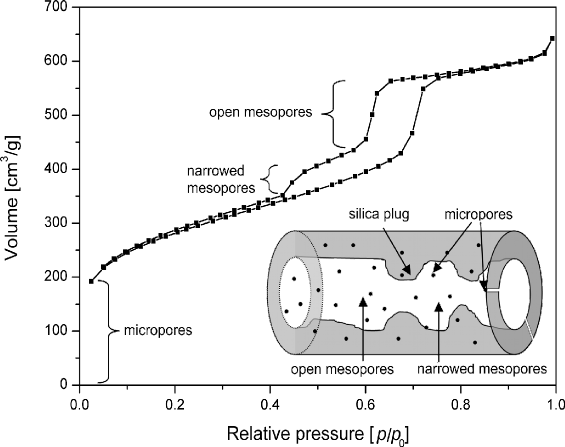
\includegraphics[width=0.90\textwidth]{Graficos/Doble-distr.png}
			       	\caption{Efecto de poros bloqueados en silice\index{silicio!oxido de} calcinada estructurada con Pluronic 123.}
			       	\label{fig:thielemann}
			   		\end{subfigure}
			   		\begin{subfigure}[t]{0.49\textwidth}
			   	    \includegraphics[width=\textwidth]{Graficos/SI_F127_simplificado_EPA.pdf}
			   	    \caption{Isoterma de adsorción\index{adsorción}/desorción de agua realizada por EPA para una \pdmF.}
			   		\end{subfigure}
					 \caption[Microscopías \pdmF\space tratamiento simplificado.]{Isotermas obtenidas para sílice mesoporosa\index{película!mesoporosa} con poros bloquedados. (a) Isoterma extradida de la publicación de Thielemann\index{Thielemann}\cite{Thielemann2011} y, (b) isoterma\index{isoterma} para sistemas \pdmF\space condensadas y extraídas por el métodos simplificado.}
					 \label{fig:F127_simplificado_EPA_2}	
				     \end{figure}

			 En los espectros de IR, para ambos sistemas de poros (figuras \ref{fig:IR_CTAB_simplificado} y \ref{fig:IR_F127_simplificado}), se observa, entre otras, el típico acoplamiento TO$_3$-LO$_3$ que resultan en un hombro a \SI{1180}{\cm^{-1}}} indicativo de una estructura porosa\cite{Innocenzi2003}. También se ha estimado el grado de condensación\index{condensación} en función de la relación en la intensidad de las bandas para $\nu_{\text{Si-O-Si/}}\nu_{\text{Si-OH}}$ y el porcentaje de extracción\index{extracción} del surfactante\index{surfactante} siguiendo la intensidad de la banda para el estiramiento C-H. Como se discutirá más adelante, ésta vibración\index{vibración} puede no solo estar asociada al surfactante\index{surfactante} sino a la esterificación\index{esterificación} de la sílice en el proceso de extracción\index{extracción} alcohólica.

			 Todos los resultados, para este y todos los tratamientos, se encuentran resumidos en la tabla \ref{tabla:resultados}.

	 \subsection{Método prolongado}

	 	 Este tratamiento se basó en prolongar el tiempo de condensación\index{condensación}. Luego de la estabilizar las \pdm\space en cámara de humedad (50 \% HR) se dejó en horno a \SI{130}{\celsius} por el término de 7 días, luego se llevó a cabo la extracción\index{extracción} del surfactante\index{surfactante}.

	 	 El resultado de este proceso fueron depósitos homogéneas sobre silicio, sin discontinuidades ni grietas y con poros bien formados para ambos surfactante\index{surfactante}s. Cuando se utilizó Au\index{oro} como soporte, solo se obtuvieron películas de buen aspecto cuando se las estructuró con F127. Para las estructuradas con CTAB se observaron grietas y sectores enteros completamente desprendidos de los electrodos. Nuevamente, al igual que en el tratamientos anterior, este hecho sugiere que la adsorción\index{adsorción} de las micelas de CTAB al oro\index{oro} impiden la adhesión de las \pdmC\space a los electrodos (figuras \ref{fig:Microscopia_F127_prolongado} y \ref{fig:Microscopia_CTAB_prolongado}).

	 	 Respecto de la caracterización por EPA, para \pdmF, se observa la misma distribución de <<doble cuello\index{cuello de poro}>> o poros bloqueados que en el caso del tratamiento simplificado (figura \ref{fig:F127_prolongado_EPA}). En cambio, los sistemas \pdmC\space sometidos a este tratamiento muestran isoterma\index{isoterma}s prácticamente idénticas al sistema calcinado, con poros de \SI{2,5}{nm} y cuello\index{cuello de poro}s de \SI{1,9}{nm} (figura \ref{fig:CTAB_prolongado_EPA}).

	 	 Los gráficos de espectroscopia\index{espectroscopia} IR para ambos sistemas de poros, F127 y CTAB (figuras \ref{fig:IR_F127_prolongado} y \ref{fig:IR_CTAB_prolongado}), muestran que la extracción\index{extracción} fue exitosa. Si bien en el caso de las \pdmC\space se ve todavía una pequeña cantidad de surfactante\index{surfactante}, la cantidad relativa al no extraído es mucho menor que en el tratamiento simplificado, indicando que la extracción\index{extracción} fue mayor. La condensación\index{condensación} también se ha mejorado, respecto del tratamiento anterior, tal como indica el aumento relativo de la vibración\index{vibración} correspondiente al estiramiento Si-O-Si, lo cual sugiere una maduración de la estructura porosa debido a la elongación en el tiempo de condensación\index{condensación}. Los valores porcentuales de ambas observaciones se pueden consultar en la tabla \ref{tabla:resultados}.

	 \subsection{Método de alto vacio\index{alto@alto vacío}}\label{sec:trat-vacio}

	     Luego del éxito parcial del tratamiento prolongado, donde se obtuvieron películas homogéneas y con arreglos de poros bien formados y con estructuras comparables a la de las películas mesoporosa\index{película!mesoporosa} calcinadas\cite{Mogilnikov2002,Fuertes2008,Rothen1945}, se hizo un tratamiento similar, en cuanto a tiempo y temperatura (7 días a \SI{130}{\celsius}), pero colocando las muestras en alto vacio\index{alto@alto vacío}, a \SI{e-5}{\milli\bar}.

		 El motivo de llevar a cabo este tratamiento fue abastecer al sistema de calor, durante un cierto tiempo, para darle oportunidad de relajar y estabilizar el cristal líquido\index{cristal líquido} y, a la vez, aplicando vacío, desplazar el equilibrio de la reacción  \ref{eq:vacio} según el principio de Le Chatelier\index{Le Chatelier}\cite{Atkins2006}, removiendo productos de reacción volátiles (H$_2$O y alcoholes) y así favorecer la condensación\index{condensación} del óxido.\cite{Zhuravlev2000}

	 		\begin{equation}
				 \schemestart 
				 Si-OH + X-O-Si 
				 \arrow{->[\scriptsize{T=\SI{130}{\celsius},P=\SI{e-5}{\milli\bar}}][\scriptsize{X=H,CH$_3$CH$_2$}]}[0,2.5] 
				 Si-O-Si + X-OH $\hspace{-0.1cm}\Big\uparrow$
				 \schemestop
				 \label{eq:vacio}
				 \end{equation}
				
		 Para sistemas \pdmF, las microscopia\index{microscopía}s ópticas muestran películas homogéneas, sin discontinuidades ni grietas mientras que las electrón\index{electrón}icas revelan la presencia de nanoporos sobre ambos sustratos, silicio\index{silicio} y oro, con poros de \SI{9}{\nm} de diámetro (ver figura \ref{fig:Microscopia_F127_vacio}). Respecto de las películas estructuradas con CTAB, presenta el mismo comportamiento que en los casos anteriores: se observa un deposito homogéneo y sin grietas cuando se depositan sobre silicio, pero se observan discontinuidades y grietas cuando se depositan sobre Au\index{oro} \ref{fig:Microscopia_CTAB_vacio}.

		 La isoterma\index{isoterma} de adsorción\index{adsorción}/desorción de H$_2$O muestra que desaparece la doble distribución\index{distribución!doble} de cuello\index{cuello de poro}s que se observó en los tratamientos anteriores para las películas estructuras con F127 (figuras \ref{fig:F127_vacio_EPA} y \ref{fig:F127_vacio_PSD}). El resultado es una isoterma\index{isoterma} tipo IV con histérisis H1, propia de sistemas con poros monodispersos uniformemente distribuidos, alcanzando un índice de refracción\index{indice@índice de refracción} de $n=1,25$ (a P/P$_s$=0\%) y una porosidad\index{porosidad} de $38\%$, valores próximos a los de un sistema calcinado. A su vez, para \pdmC, el resultado por PEA es una isoterma\index{isoterma} que devuelve una porosidad\index{porosidad} (44 \%) y un índice de refracción\index{indice@índice de refracción} ($1,393$) prácticamente igual al del calcinado (figura \ref{fig:CTAB_vacio_EPA}) con una distribución de tamaño de poros y cuello\index{cuello de poro}s (figura \ref{fig:CTAB_vacio_PSD})comparable con la reportada por Boissiere\index{Boissiere}\cite{Boissiere2005}.

		 De los espectros IR  (figuras \ref{fig:IR_F127_vacio} y \ref{fig:IR_CTAB_vacio}) se puede concluir que que la extracción\index{extracción} del surfactante\index{surfactante} (ya sea para las películas estructuradas con F127 o estructuradas con CTAB) fue buena, pero no total, obteniendo valores de extracción\index{extracción} por encima del 85\%. Para ambos sistemas la relación de intensidades $\nu{\text{Si-O-Si/}}\nu{\text{Si-OH}}$, así como un ángulo de contacto\index{angulo@ángulo de contacto} alto, demuestran que se trata de una estructura porosa con pared bien condensada. Los valores se encuentran en la tabla \ref{tabla:resultados}.

		 %Fijarse de algun trabajo de mesosporoso con angulo de contacto para poner de referencia.

	 \subsection{Método ácido}

	 	 Al\index{aluminio}gunos autores proponen que un medio fuertemente ácido\index{acido@ácido} (pH$<1$) favorece la hidrólisis\index{hidrolisis@hidrólisis} del alcóxido y la condensación\index{condensación} de los grupo siloxano \cite{Soler-Illia2011,Doshi2000a,Huo1996,Boissiere2000,Beck1992}. Las películas depositadas, estabilizadas en cámara de humedad y  parcialmente condensadas a \SI{130}{\celsius}, tal como se explica en la sección \ref{sec:cond_y_extr}, pág. \pageref{sec:cond_y_extr}, fueron expuestos a una atmósfera de HCl\index{acido@ácido!clohídrico} durante \SI{15}{\minute}. 

		 En las microscopia\index{microscopía}\index{microscopía}s para las \pdm\space sometidas a este método (ya sean estructuradas con F127 como con CTAB) se observan grietas y discontinuidades cuando se depositaron sobre electrodos de Au\index{electrodo!de Au} (figuras \ref{fig:Microscopia_F127_acido} y \ref{fig:Microscopia_CTAB_acido}). Este hecho se ha atribuido a una condensación\index{condensación} rápida, catalizada por el medio extremadamente ácido. Al\index{aluminio} no presentar buena adherencia\index{adherencia} sobre el sustrato, las películas de sílice se contraen en todas las direcciones, y no solo en la dirección normal a la superficie\index{superficie}, como ocurre en las \pdm\space depositadas sobre silicio, donde las fuerzas de adherencia\index{adherencia} al sustrato\index{sustrato} priman por sobre las fuerzas contracción en el plano\cite{Sakatani2006,Boissiere2005,Guillemin2010}. En ese caso las películas quedan bien formadas y homogéneas en toda el área de la muestra para ambos surfactante\index{surfactante}s. Se ha observado por microscopia\index{microscopía} electrón\index{electrón}ica que para los sistemas \pdmF\space (\ref{fig:Microscopia_F127_acido}) los  poros están casi unidos formando una especie de poro\index{poro} elongado, propio de una estructura \textit{p6mm}\cite{GonzalezSolveyra2017}. 
	
		 Esta morfología superficial de poros elongados se corroboró por PEA (figura \ref{fig:F127_acido_EPA}). Al\index{aluminio}lí se observa, en la isoterma\index{isoterma} de adsorción\index{adsorción}/desorción de agua, una doble distribución\index{distribución!doble} de cuello\index{cuello de poro}s donde predominan cuello\index{cuello de poro}s de diámetro grandes, casi del mismo tamaño que los poros, coincidiendo con la observación por microscopia\index{microscopía} electrón\index{electrón}ica.
		 La isoterma\index{isoterma} de adsorción\index{adsorción}/desorción de agua para \pdmC\space muestra que se trata de sistemas con una porosidad\index{porosidad} del 38\% y un índice de refracción\index{indice@índice de refracción} $n=1.23$, al igual que en el caso del F127 apenas superior que en el caso de lo sistemas calcinados.
		
		 En lo referente a la etapa de extracción\index{extracción}, se observa por espectroscopia\index{espectroscopia} IR, que fue efectiva para ambos sistemas de poros, alcanzando un alto porcentaje de extracción\index{extracción}, $91,5$\% para CTAB y $85,7$\% para F127 (figuras \ref{fig:IR_CTAB_acido} y \ref{fig:IR_F127_acido}).  	
				
	 \subsection{Método alcalino}

	 	 El último de los tratamientos experimentados en pos de conseguir depositar y condensar peliculas mesoporosa\index{película!mesoporosa} de óxido de silicio\index{silicio!oxido de}\index{silicio} a bajas temperatura fue el tratamiento en medio básico. Análogamente al realizado en medio ácido, se basa en someter a las películas a un medio de pH\index{pH} extremo (pH$>12$), el cual, según algunos autores \cite{Soler-Illia2011,Huo1996,Ichinose2002,GonzalezSolveyra2017}, cataliza los procesos de hidrólisis\index{hidrolisis@hidrólisis} del TEOS. En este caso las películas, luego de la estabilización en humedad, fueron colocadas en una atmósfera de NH\index{amoniaco}$_3$ durante \SI{15}{\minute}. 

		 Los depósitos obtenidos sobre Au\index{oro} presentan grandes grietas y zonas muy fraccionadas para ambos sistemas porosos, \pdmF\space y \pdmC. Esta observación se atribuye nuevamente a la violenta condensación\index{condensación} catalizada por el medio, en este caso fuertemente alcalino. Sobre silicio\index{silicio} las \pdm\space resultaron en depósitos homogéneos y de buen aspecto tanto por microscopia\index{microscopía}\index{microscopía}\index{microscopía!óptica} como electrón\index{electrón}ica (figuras \ref{fig:Microscopia_F127_basico} y \ref{fig:Microscopia_CTAB_basico}).

		 En las elipsoporosimetría\index{elipsoporosimetría ambiental} realizadas, se observa para el sistema \pdmF\space una doble distribución\index{distribución!doble} de cuello\index{cuello de poro}s muy similar a la obtenida por el tratamientos en medio ácido, pero en este caso el índice de refracción\index{indice@índice de refracción} fue de $n=1.22$ (a P/P$_s$ = 0) el cual es prácticamente idéntico al que presentan los sistema calcinado (ver figura \ref{fig:F127_basico_EPA} y tabla \ref{tabla:resultados}). Para poros estructurados con CTAB las mediciones por PEA muestran una isoterma\index{isoterma} tipo IV, con histérisis H1, resultando en un sistema muy poroso ($40\%$) y un índice de refracción\index{indice@índice de refracción} $n=1,22$.
	
		 Los espectros IR para ambos surfactante\index{surfactante}s (figura \ref{fig:IR_CTAB_basico} para CTAB y \ref{fig:IR_F127_basico} para F127) muestran una ruptura en el aspecto del típico hombro (acoplamiento LO$_3$-TO$_3$, en \SI{1180}{\per\cm}) para estructuras de sílice mesoporosas \cite{Olsen1989,Innocenzi2003,Angelome2008}. Esto sugiere un colapso de la organización de poros en la nanoescala\index{nanoescala}, debido a la disolución parcial de la sílice, catalizada por el medio básico. Si bien el medio básico\index{básico} acelera la hidrólisis\index{hidrolisis@hidrólisis} del TEOS, también aumenta la tasa de disolución del SiO$_2$.\cite{Mazer1994,Niibori2000,Gorrepati2010}

	 \subsection{Comparación de resultados}
	 		
	 		Se presentan en la tabla \ref{tabla:resultados} todos los resultados, obtenidos para cada sistema de poros, \pdmF\space y \pdmC, por cada una de las técnicas de caracterización empleadas. 

	 		La tabla se compone de varias columna; una para microscopia\index{microscopía} donde se coloca el aspecto que presentan las diferentes \pdm\space tanto sobre oro\index{oro} como sobre silicio; otra con resultados de poroelipsometría\index{poroelipsometría ambiental} ambiental y los valores que extraídos de las isoterma\index{isoterma}s: diámetro de poro\index{poro} ($\varnothing_p$), de cuello\index{cuello de poro}($\varnothing_c$), porosidad\index{porosidad} (\%P), espesor\index{espesor} ($e$) e índice de refracción\index{indice@índice de refracción} de la pared ($n$); otra para los resultados de FTIR\index{FTIR} donde se ha volcado el porcentaje de extracción\index{extracción} del surfactante\index{surfactante} y la relación de intensidad picos $\nu_{\text{Si-O-Si/}}\nu_{\text{Si-OH}}$; una más para la accesibilidad\index{accesibilidad} al electrodo de sonda\index{sonda}s EQ; otra para el ángulo de contacto\index{angulo@ángulo de contacto} ($\theta$) y una última reservada para observaciones generales.  
	 		
	 		\pagebreak

	
			 \begin{table}[ht!]
			 \caption[Comparación de resultados \pdm]{Resumen de resultados obtenidos por cada una de las técnicas de caracterización, para cada uno de los métodos pos-depósito aplicados a \pdm.}
			 \label{tabla:resultados}
		 	 \begingroup
		 	 \subcaption{Parte A: Microscopía, elipsoporosimetría\index{elipsoporosimetría ambiental} y ángulo de contacto\index{angulo@ángulo de contacto}.}
			 \endgroup
			 \begin{tabular}{>{\raggedright\arraybackslash}m{1.5cm}>{\centering\arraybackslash}m{0.7cm}>{\centering\arraybackslash}m{0.7cm}>{\centering\arraybackslash}m{0.1cm}>{\centering\arraybackslash}m{0.75cm}>{\centering\arraybackslash}m{0.75cm}>{\centering\arraybackslash}m{0.75cm}>{\centering\arraybackslash}m{0.75cm}>{\centering\arraybackslash}m{0.75cm}>{\centering\arraybackslash}m{0.98cm}} 
			 \toprule
				 \multirow{2}{*}{Método}& \multicolumn{2}{c}{Microscopia$^*$}&&\multicolumn{5}{c}{Elipsoporosimetría} & AC \\
    			   		& Si & Au\index{oro} & & $\varnothing_p$ & $\varnothing_c$ & \%P & $e$(nm) & $n(\lambda\index{longitud de onda})^\mathsection$ &$\theta^\circ$\\ \midrule
    			 
    			 CalSC   &\checkmark&\xmark&& 2,5 & 2,0 & 42 & 345 & 1,384 & 33,2 \\ 
  	 	         CalSF   &\checkmark&\checkmark&& 8,2 & 4,4 & 38 & 207 & 1,391 & 20,0 \\ \midrule
  	 	         SimSC   &\checkmark&\xmark&& 2,2 & 2,0 & 30 & 308 & 1,389 & 41,2 \\ 
			     SimSF   &\checkmark&\checkmark&& 7,5 & \hspace{1.5mm}3,9$^\dagger$& 30 & 211 & 1,390 & 36,4 \\ \midrule
				 ProSC   &\checkmark&\xmark&& 2,5 & 2,0 & 41 & 338 & 1,375 & 44,5 \\ 
				 ProSF   &\checkmark&\checkmark&& 8,0 & \hspace{1.5mm}4,0$^\dagger$  & 39 & 212 & 1,381 & 22,7 \\ \midrule
				 VacSC   &\checkmark&\xmark&& 2,2 & 1,7  & 44 & 381 & 1,393 & 65,5 \\ 
				 VacSF   &\checkmark&\checkmark&& 9,0 & 4,0  & 38 & 223 & 1,383 & 42,5 \\
				 VacZSF  &\checkmark&\checkmark&&  -  &  -	 & -  &  -  &    -  &   -  \\ \midrule	
				 ÁciSC   &\checkmark&\xmark&& 2,0 & 1,6  & 37 & 340 & 1,386 & 46,0 \\ 
				 ÁciSF   &\checkmark&\xmark&& 5,7 & \hspace{1.5mm}2,1$^\dagger$  & 31 & 191 & 1,399 & 28,2 \\ \midrule
				 Al\index{aluminio}cSC   &\checkmark&\xmark&& 2,3 & 1,6  & 46 & 383 & 1,396 & 47,6 \\ 
				 Al\index{aluminio}cSF   &\checkmark&\xmark&& 8,0 & 2,1$^\dagger$ & 32 & 225 & 1,374 & 24,5 \\
			\bottomrule
			\end{tabular}
		    \begingroup
		    \subcaption{Parte B: Accesibilidad de sonda\index{sonda}s EQ, espectroscopía IR y observaciones.}
			\endgroup
			\begin{tabular}{>{\raggedright\arraybackslash}m{1.5cm}>{\centering\arraybackslash}m{1cm}>{\centering\arraybackslash}m{1cm}>{\centering\arraybackslash}m{1.6cm}>{\raggedright\arraybackslash}m{4.9cm}} 
			\toprule
				 \multirow{2}{*}{Método}& \multicolumn{2}{c}{FTIR} & Señal EQ$^\ddagger$ & Observaciones generales\\
    			   		 & $\frac{\nu{\text{Si-O-Si}}}{\nu{\text{Si-OH}}}$ & \%$_{\text{ext}}$  \\ \midrule

    			 CalSC   & 1,08  & 100  & \checkmark & falta de adherencia\index{adherencia} en Au\index{oro}  \\ 
  	 	         CalSF   & 0,77  & 100  & \checkmark &   \\ \midrule
  	 	         SimSC   & 0,67  & 72,7 & \xmark & falta de adherencia\index{adherencia} en Au\index{oro}  \\ 
			     SimSF   & 0,53  & 70,4 & \xmark & doble cuello\index{cuello de poro} \\ \midrule
				 ProSC   & 0,80  & 87,7 & \xmark & falta de adherencia\index{adherencia} en Au\index{oro}  \\ 
				 ProSF   & 0,78  & 97,0 & \xmark & doble cuello\index{cuello de poro} \\ \midrule
				 VacSC   & 0,88  & 87,5 & \checkmark & falta de adherencia\index{adherencia} en Au\index{oro}  \\ 
				 VacSF   & 0,78  & 88,0 & \checkmark &   \\ 
				 VacZSF  &   -   &   -  & \checkmark &   \\ \midrule
				 ÁciSC   & 0,80  & 91,5 & \xmark & falta de adherencia\index{adherencia} en Au\index{oro}  \\ 
				 ÁciSF   & 0,81  & 85,7 & \xmark & doble cuello\index{cuello de poro}, poros <<elongados>>  \\ \midrule
				 Al\index{aluminio}cSC   & 0,99  & 94,4 & \xmark & \multirow{2}{*}{pérdida de la estructura porosa} \\ 
				 Al\index{aluminio}cSF   & 0,98  & 91,2 & \xmark &   \\
			\bottomrule
			\end{tabular}\vspace*{2pt}
			\footnotesize{$^*$se evalúa la adherencia, presencia de grietas o discontinuidades y la morfología superficial de los poros.}\\
			\footnotesize{$^\mathsection$ Valores correspondientes al $n$ calculado para las paredes de los sistemas mesoporosos a $\lambda\index{longitud de onda}=$\SI{600}{\nm}; $n_{SiO_2}=1,45$.}\\
			\footnotesize{$^\dagger$ Sistemas con doble distribución\index{distribución!doble} de cuello\index{cuello de poro}s, se reporta la población más abundante.}\\
			\footnotesize{$^\ddagger$ Se refiere a la accesibilidad\index{accesibilidad} de la sonda\index{sonda} al electrodo.}
		    %\footnotesize{$^*$se evalúa la adherencia, presencia de grietas o discontinuidades y la apariencia superficial de los poros.}
			
			\end{table}					 	  
			
\section{Discusión sobre los métodos}
		
			Luego de depositar, sintetizar, llevar a cabo los tratamientos y caracterizar las distintas películas, se hace aquí, una discusión de los resultados sobre cada sistema. El resultado de la discusión y el análisis llevará a elegir uno o más tratamientos adecuados para la fabricación de los sensores\index{sensor} basados en películas mesoporosas.

	\subsection{Sobre los sustratos}

			Es importante destacar que uno de los objetivos principales de este trabajo es depositar las \pdm\space sobre un sustrato\index{sustrato} óptimo para hacer reacciones electroquímica\index{electroquimico}s\index{electroquimico}. En este caso se eligió oro. Sin embargo, para llevar a cabo numerosas caracterizaciones, entender las bases de algunos comportamientos y comparar con la literatura, fue necesario hacer depósitos sobre silicio, ya que además se utiliza una capa dieléctrica de SiO$_2$.

			Los sistemas que usaron CTAB y fueron depositados sobre Au\index{oro} presentaron todos grietas, fracturas y discontinuidades, como ya fué mencionando en reiteradas ocasiones, esto es consecuencia de la adsorción\index{adsorción} superficial del Br sobre el Au. 

			Hubo dos métodos en particular, el tratamientos en medio ácido\index{acido@ácido} y el tratamientos en medio básico, que mostraron el mismo comportamiento independientemente del surfactante\index{surfactante} utilizado. Ambos presentan grietas a lo largo de toda la película sobre sustrato\index{sustrato} de Au. Esto es resultado de dos factores combinados; la baja adherencia\index{adherencia} sobre sustrato\index{sustrato} de Au\index{oro} (a los sistemas con CTAB se le suma la adsorción\index{adsorción} del surfactante\index{surfactante} al sustrato) y la violenta condensación\index{condensación} catalizada por el medio, ya se sea ácido\index{acido@ácido} o básico. Esto lleva a una contracción en todas direcciones ya que la fuerza de adherencia\index{adherencia} al Au\index{oro} es menor que la fuerza de contracción en el plano de la película, lo cual genera las discontinuidades y grietas en las \pdm. No ocurre lo mismo cuando el sustrato\index{sustrato} es silicio, donde la adherencia\index{adherencia} es fuerte. En este caso la contracción es uniaxial (como es lo habitual para sistemas calcinados) y sólo ocurre en el eje normal a la superficie\index{superficie}, resultando en depósitos continuos y homogéneos.

			El resto de los tratamientos sobre Au\index{oro} para F127 resultó en depósitos homogéneos.

			Respecto de la adherencia\index{adherencia} sobre silicio, todos lo tratamientos fueron exitosos para ambos surfactante\index{surfactante}s.

	\subsection{Sobre la condensación\index{condensación}}

		Una de las dos técnicas utilizadas para evaluar la condensación\index{condensación} fue elipsoporosimetria ambiental (PEA). De esta técnica podemos extraer datos como el índice de refracción\index{indice@índice de refracción} del SiO$_2$ poroso ponderando su porosidad, según la aproximación de Bruggeman\index{Bruggeman}, la cuál debe satisfacer la ecuación \ref{eq:bruggeman} \cite{Bruggeman1935}. Este valor, comparado con el sistema calcinado, nos da una idea de cuán condensada está la película. 

		También extraemos de las isoterma\index{isoterma}s la porosidad\index{porosidad} y el diámetro de poro\index{poro} y cuello\index{cuello de poro}. Todos los métodos ensayados para ambos surfactante\index{surfactante}s resultaron en películas porosas. Sin embargo para el F127, muchos de los tratamientos (simplificado, ácido\index{acido@ácido} y básico) presentaron doble distribución\index{distribución!doble} de cuello\index{cuello de poro}s. Para todos los tratamientos los índices de refracción dan valores comparables con óxidos mesoporosos calcinados, indicando una condensación\index{condensación} similar a estos. En las figuras \ref{fig:todos_EPA_F127} y \ref{fig:todos_EPA_CTAB} se comparan todas las isoterma\index{isoterma}s para cada uno de los sistemas, estructurado con CTAB y con F127. En la tabla \ref{tabla:resultados} se resumen los valores cuantitativos extraídos de dichas isoterma\index{isoterma}s para cada uno de los sistemas.

			\begin{figure}[!th]
		 	   	   \begin{center}
		 	   	   \includegraphics[width=0.85\textwidth]{Graficos/SI_CTAB_todos_EPA.pdf}
			   	   \caption[Comparación PEA tratamientos alternativos (CTAB)]{Comparación de las isoterma\index{isoterma}s para todos los tratamientos pos-depósito para \pdmC\space. Destacan los altos índices de refracción para los tratamientos simplificado y en medio ácido.}
				   \label{fig:todos_EPA_CTAB}	
				   \end{center}
				   \end{figure}
						   
			\begin{figure}[!th]
		 	   	   \begin{center}
		 	   	   \includegraphics[width=0.85\textwidth]{Graficos/SI_F127_todos_EPA.pdf}
			   	   \caption[Comparación PEA tratamientos alternativos (F127)]{Comparación de las isoterma\index{isoterma}s para todos los tratamientos pos-depósito para \pdmF\space. Se destacan la doble distribuciones de cuello\index{cuello de poro}s para algunos de ellos.}
				   \label{fig:todos_EPA_F127}	
				   \end{center}
				   \end{figure}	

		\pagebreak		   
				   
		La otra técnica utilizada para evaluar la condensación\index{condensación} fue espectroscopia\index{espectroscopia} IR. Para ello se calculó la relación existente entre la intensidad de picos correspondiente a las vibraciones\index{vibración} $\nu{\text{Si-O-Si}}$ y $\nu{\text{Si-OH}}$ \cite{Pai1986,Innocenzi2003}. Un número más grande indica mayor cantidad de enlaces Si-O-Si, por lo tanto mayor grado de condensación\index{condensación}. Se observa en la tabla \ref{tabla:resultados} que los mayores valores corresponden a los sistemas calcinados y los menores a los sistemas en lo que solo se estabilizó a \SI{130}{\celsius} (método simplificado). Los valores obtenidos para el resto de los tratamientos se encuentran próximos a los valores correspondientes a sistemas calcinados, lo cual sugiere un buen grado de condensación\index{condensación}.  Otra banda importante es el hombro de LO$_3$ (\SI{1180}{\per\cm}) formado a mayores frecuencia de TO$_3$, característico de estructuras porosas de SiO$_2$. Esta señal se debe al acoplamiento longitudinal/transversal de los modos TO$_3$ y LO$_3$ ocasionada por la dispersión de la luz en la red porosa, que estimula el modo longitudinal el cual habitualmente no se excita cuando se mide en modo trasmisión\cite{Innocenzi2003,Lange1990,Lange1989}. La ausencia de este acoplamiento sugiere un sistema poco poroso o más denso. Esto sugiere, junto a otros indicios, al colapso parcial de la estructura porosa. En la tabla \ref{tabla:resultados} se muestras los valores cuantitativos respecto de estas bandas.	   

	\subsection{Sobre la extracción\index{extracción}}

		Al utilizar métodos alternativos a la calcinación\index{calcinación} se requirió una etapa de extracción\index{extracción} para eliminar el surfactate. En todos los caso se llevó a cabo en 2-propanol\index{propanol@2-propanol} a reflujo\index{reflujo}. Si bien fue exitosa en la mayoría de los casos, con valores de extracción\index{extracción} por encima del 85\%, siempre se observa una pequeña banda correspondiente a la vibración\index{vibración} C-H en el IR. Dicha banda puede provenir tanto del surfactante\index{surfactante} como de es un intercambio del hidroxilo por el propanol según:
			\begin{equation}
				 \schemestart 
				 Si-OH + OH-CH$_2$CH$_3$ 
				 \arrow{<=>}[0,1.5] 
				 Si-O-CH$_2$CH$_3$ + H$_2$O
				 \schemestop
				 \label{eq:prolilo}
				 \end{equation}
		Por este motivo, luego de la extracción\index{extracción} con 2-propanol, se realizó un enjuague de las muestras con H$_2$O acidificada con HCl\index{acido@ácido!clohídrico} (pH$\approx 2$) para poder completar la extracción\index{extracción}, ya sean residuos de surfactante\index{surfactante} o propanol ligado.
			
			\begin{figure}[ht!]
			\begin{center}
			\includegraphics[width=0.74\textwidth]{Graficos/IR_F127_vacio_AGUA.pdf}
			\caption[FTIR extracción\index{extracción} agua ácida.]{IR para cada etapa de eliminación\index{eliminación} del surfactante\index{surfactante} correspondiente a una \pdmF\space sintetizada por el método de alto vacio\index{alto@alto vacío}.}
			\label{fig:IR_agua}
			\end{center}
			\end{figure}

		En la figura \ref{fig:IR_agua} se muestra una película delgada \index{película!delgada}de sílice, estructurada con F127, y preparado por el método de alto vacio\index{alto@alto vacío}. Al\index{aluminio}lí donde se comparan tres espectros IR para cada etapa; la película antes de extraer el surfactante\index{surfactante}, luego de extraerlo con 2-propanol\index{propanol@2-propanol} y, luego de extraerlo con el alcohol y seguido de un enjuague en agua acidificada. Se ve como con el enjuague en agua ácida disminuye la señal correspondiente a la vibración\index{vibración} C-H, que aparece ya sea por restos de surfactante\index{surfactante} y/o de la esterificación\index{esterificación} del 2-propanol.

	\subsection{Sobre la respuesta electroquímica\index{electroquimico}}\label{sec:acc_eq}

	  Una parte fundamental en la fabricación de las \pdm\space y su potencial uso para sensores\index{sensor} electroquímico\index{electroquimico}s\index{electroquimico} es la accesibilidad\index{accesibilidad} de moléculas dentro de la red porosa. Ya se demostró, en la sección \ref{sec:acc}, pág. \pageref{sec:acc} que el \aminorutenio\space es capaz de difundir en sistemas calcinados a través de los poros hasta la superficie\index{superficie} del electrodo, donde tiene lugar la reacción electroquímica\index{electroquimico}. Se debe evaluar, entonces,  la accesibilidad\index{accesibilidad} en sistemas de poros no calcinados. Los mediciones electroquímica\index{electroquimico}s\index{electroquimico} se llevaron a cabo en películas depositadas, condensadas y extraídas con el tratamiento de alto vacio\index{alto@alto vacío}, ya que es el que mostró las mejores condiciones de adherencia\index{adherencia} al Au, condensación\index{condensación} y distribución de poros para usar en sensores\index{sensor} EQ. 

	  		\begin{figure}[ht!]
		 	
		 	\begin{subfigure}[t]{0.5\textwidth}
		          	\includegraphics[width=\textwidth]{Graficos/Ru-F127-CNEA-Calcinado-0-1.pdf}
		          	\vspace*{-6mm}
		         	\caption{Ciclos de VC para \ru\space \SI{0.1}{\milli\Molar}.}
		          	\vspace*{3mm}
		          	\end{subfigure}
		    \begin{subfigure}[t]{0.5\textwidth}
		          	\includegraphics[width=\textwidth]{Graficos/Ru-F127-INTI-BajaT-0-1.pdf}
		         	\vspace*{-6mm}
		         	\caption{Ciclos de VC para \ru\space \SI{0.1}{\milli\Molar}.}
		      		\vspace*{3mm}
		      		\end{subfigure}
		    \begin{subfigure}[t]{0.5\textwidth}
		          	\includegraphics[width=\textwidth]{Graficos/Ru-F127-CNEA-Calcinado-1.pdf}
		         	\vspace*{-6mm}
		         	\caption{Ciclos de VC para \ru\space \SI{1}{\milli\Molar}.}
		            \vspace*{3mm}
		            \end{subfigure}
		    \begin{subfigure}[t]{0.5\textwidth}
		          	\includegraphics[width=\textwidth]{Graficos/Ru-F127-INTI-BajaT-1.pdf}
		         	\vspace*{-6mm}
		         	\caption{Ciclos de VC para \ru\space \SI{1}{\milli\Molar}.}
		    		\vspace*{3mm}
		    		\end{subfigure}
		      	 	\caption[Voltagrama comparativo SF calcinados/alto vacío I]{Voltametrías cíclicas donde se compara la accesibilidad\index{accesibilidad} de una sonda\index{sonda} electroquímica\index{electroquimico} sobre \pdmF\space con dos tratamientos pos-depósito diferentes; (a) y (c) por calcinación\index{calcinación} a (\SI{350}{\celsius}) y, (b) y (d) por el método de alto vacio\index{alto@alto vacío} (\SI{130}{\celsius}, 7 días, P=\SI{e-5}{\milli\bar}). Todas las VC fueron realizadas en una solución \SI{0.1}{\Molar} de KCl a \SI{50}{\milli\volt\per\second}.}
		      		\label{fig:comp-calc-vacio}
	      \end{figure}

	  En la figura \ref{fig:comp-calc-vacio} se exponen las voltametrías cíclicas comparando \pdmF\space condensadas por calcinación\index{calcinación} y por el método de alto vacio\index{alto@alto vacío}, a dos concentraciones de sonda\index{sonda} diferentes. Los voltagramas están compuestos por ciclos consecutivos de voltametrías cíclicas hasta llegar a un máximo donde ya no varía la respuesta. Este respuesta corresponde al ingreso y adsorción\index{adsorción} de la sonda\index{sonda} en las \pdm, hasta llegar a la saturación. Este comportamiento es materia central del capitulo siguiente donde se lleva a cabo una profunda discusión sobre los fenómenos de transporte\index{transporte} dentro de los poros.

      Si bien la capacidad de adsorción\index{adsorción} es prácticamente igual (la concentración dentro de los poros área de la curva azul), ya sea que se trate del sistema calcinado o del sistema de alto vacio\index{alto@alto vacío}, el mecanismo de adsorción\index{adsorción} parece ser diferente. En los calcinados la respuesta del primer ciclo se corresponde con la de una sonda\index{sonda} en un electrodo de Au\index{electrodo!de Au}\index{oro} sin \pdm, para luego evolucionar en la respuesta típica de un adsorbido. En cambio, en los sistemas de alto vacio\index{alto@alto vacío}, los primeros ciclos no dan respuesta, y, conforme la sonda\index{sonda} ingresa en los poros, la respuesta aumenta y hasta ser prácticamente igual a la del sistema calcinado. Este comportamiento sugiere que la accesibilidad\index{accesibilidad} no es igual para ambos sistemas. Los calcinados son sistemas más <<abiertos>> o mas comunicados. En los sistemas condensados a bajas temperaturas la difusión\index{difusión} de la sonda\index{sonda} al electrodo parece esta impedida, y la respuesta aumenta conforme aumenta la concentración de sonda\index{sonda} dentro de los poros. En resumen, en los sistemas calcinados la difusión\index{difusión} es más rápida que la adsorción\index{adsorción} y en los de alto vacio\index{alto@alto vacío} la difusión\index{difusión} esta impedida y solo se ve señal a medida que se adsorbe, a pesar de que la capacidad de adsorción\index{adsorción} es igual para ambos métodos.

      Esta diferencia de accesibilidad\index{accesibilidad} de los sistemas calcinados respectos de los sistemas de alto vacio\index{alto@alto vacío} también se hizo evidente cuando se utilizó ferroceno metanol\index{ferroceno metanol} como sonda\index{sonda}. Esta sonda\index{sonda} es neutra, por lo tanto no debería verse influenciada por la carga dentro de las películas. En la figura \ref{fig:fcOH_accesibilidad} se compara la respuesta de un \pdmF\space condensado y extraído por el método de alto vacio\index{alto@alto vacío} y un sistema \pdmF\space calcinado. Si bien ambos sistemas demostraron ser accesibles, los sistemas condensados a bajas temperaturas da un respuesta propia de un sistema limitado por difusión\index{difusión}. En el capítulo \ref{chap:Electroquimica} se discute y analiza en profundidad  los resultados de transporte\index{transporte} del ferroceno metanol\index{ferroceno metanol} en sistemas \pdmF, así como cálculos de constantes de difusión\index{difusión}.

      		\begin{figure}[ht!]
		 	\begin{subfigure}[t]{0.5\textwidth}
		          	\includegraphics[width=\textwidth]{Graficos/Acc-FcOH-Calcinado.pdf}
		          	\end{subfigure}
		    \begin{subfigure}[t]{0.5\textwidth}
		          	\includegraphics[width=\textwidth]{Graficos/Acc-FcOH-BajaT.pdf}
		         	\end{subfigure}
		         	\caption[Voltagrama comparativo SF calcinados/alto vacío II]{Voltametrías para \fc\space \SI{1}{\milli\Molar} en \SI{100}{\milli\Molar} de KCl realizada a \SI{50}{\volt\per\second} contra ESC. Izquierda: sobre sistemas \pdmF\space calcinados. Derecha: sobre sistemas \pdmF\space condensados por el método de alto vacio\index{alto@alto vacío} y extraído con 2-propanol\index{propanol@2-propanol} y agua.}
		         	\label{fig:fcOH_accesibilidad}
		    \end{figure}     	

\section{Conclusiones parciales}
	
	En este capítulo se presentan los resultados obtenidos durante el proceso de fabricación, desarrollo y caracterización de películas delgadas mesoporosas de óxido de silicio\index{silicio!oxido de}\index{silicio} con potencial uso en sensores\index{sensor} electroquímico\index{electroquimico}s\index{electroquimico}.
	
	Los soles, precursor\index{precursor}es de las \pdm, se depositaron exclusivamente por \textit{spin-coating}\index{spin@\textit{spin-coating}}, previendo la futura integración a los procesos propios de la industria electrón\index{electrón}ica. La organización espacial de los poros se llevó a cabo con dos agentes moldeantes, CTAB y F127, sobre diferentes sustratos: silicio, vidrio\index{vidrio} y oro. Se ajustó el espesor\index{espesor} entre 200 y \SI{250}{\nm}, el cuál se consideró óptimo para obtener \pdm\space sin fracturas ni discontinuidades; y frente a los problemas de adherencia\index{adherencia} a los electrodos se utilizaron dos estrategias: modificación química y optimización del diseño de los electrodos. 

	Una vez adquirida la experiencia para depositar y condesar por calcinación\index{calcinación} \pdm\space sobre electrodos, con poros accesibles, sin discontinuidades y con buena adherencia, se realizó un trabajo sistemático de métodos pos-depósito para obtener \pdm\space a temperaturas menores a \SI{130}{\celsius}. Para ello se realizó un trabajo sistemático y metódico sobre el estudio y desarrollo de procesos pos-depósito. En total fueron cinco los procesos desarrollados: simplificado, prolongado, alto vacio\index{alto@alto vacío}, ácido\index{acido@ácido} y alcalino.

	Los resultados muestran que cualquiera de los métodos es plausible de ser usado para obtener \pdm, con poros accesibles, y porosidades entre 30\% y 45\%. Sin embargo, este trabajo tiene por objetivo utilizar estas películas como elemento activo permeoselectivo incorporado en sensores. Para ello no basta solo con obtener películas mesoporosas sobre silicio\index{silicio} o vidrio\index{vidrio} (sistemas más clásicos), sino que hay que depositarlas y condensarlas sobre electrodos que permitan una detección electroquímica\index{electroquimico} confiable, como Au\index{oro} o Pt\index{platino}. También es preciso mantener, durante todo el proceso de síntesis, la temperatura por debajo de los \SI{150}{\celsius} para evitar procesos difusivos, como discutiremos en el capítulo \ref{chap:Microfabricacion}.

	Las películas estructuras con F127 mostraron dificultades a la hora de obtener distribuciones homogéneas de poro\index{poro} y cuello\index{cuello de poro} para los tratamientos simplificado, prolongado, ácido\index{acido@ácido} y básico. Sin embargo con tiempos de estabilización prologados y en alto vacio\index{alto@alto vacío} resultaron homogéneas en todo sentido, tanto en el deposito en sí, como en un única distribución de cuello\index{distribución!de cuello}\index{cuello de poro} y poro. Este hecho sugiere que el tiempo de estabilización prolongado sumado al alto vacio\index{alto@alto vacío} (que favorece la reacción de condensación\index{condensación}) ayudan a controlar la condensación\index{condensación} y la organización espacial de los poros, obteniendo sistemas de un buen grado de condensación\index{condensación} con poros y cuello\index{cuello de poro}s uniformemente distribuidos.

	No fue posible obtener depósitos continuos sobre Au\index{oro} en películas estructuras con CTAB. Esto se debe a las limitaciones de adherencia\index{adherencia} sobre Au, sumado a la adsorción\index{adsorción} del CTAB sobre la superficie\index{superficie} del mismo. A pesar de ello, los métodos desarrollados sobre silicio\index{silicio} demostraron ser parcialmente exitosos en todos los casos.

	De los cinco métodos desarrollados, sólo el de alto vacio\index{alto@alto vacío} resulto ser apto para utilizar indistintamente CTAB o F127. Este resultado resulta interesante en sí, ya que, si bien las películas con CTAB sobre Au\index{oro} no adhieren, es importante saber que el proceso de condensación\index{condensación} y extracción\index{extracción} es compatible con este tipo de películas, ya que permitiría combinar dispositivos multicapas mixtos de CTAB y/o F127 en un solo proceso de fabricación.

	El diagrama de la figura \ref{fig:flujo-trabajo} muestra el flujo de trabajo para el desarrollo de películas mesoporosas de óxido de silicio\index{silicio!oxido de}\index{silicio} a bajas temperaturas sobre electrodos de Au\index{electrodo!de Au} y las dificultades asociadas.

		\begin{figure}[!ht]
			\begin{center}
			\includegraphics[width=0.85\textwidth]{Esquemas/arbol-problemas.pdf}
			\caption[Flujo de trabajo para obtener electrodos con películas mesoporosa]{Diagrama árbol donde se muestra las etapas y tratamientos utilizadas con sus problemas asociados, para lograr fabricar electrodos recubiertos con películas delgadas meosoporosas de óxido de silicio\index{silicio!oxido de}}
			\label{fig:flujo-trabajo}
			\end{center}
			\end{figure}	
	
	Por supuesto el tema principal es que, a diferencia de los métodos existentes hasta ahora, en ninguno de los procesos la temperatura se eleva mas de \SI{130}{\celsius}. Evitar la calcinación\index{calcinación} permite trabajar sobre sustratos térmicamente lábiles, como polímeros, y evitar procesos difusivos en las interface\index{interface}s electrodos-mesoporoso. 

	Si se piensa en sensores\index{sensor} y procesos de fabricación complejos, que involucren una diversidad de etapas de fabricación, se podría usar cualquiera de los métodos desarrollados, eligiendo adecuadamente según el propósito que se persigue. Por ejemplo, si se desea funcionalizar las películas con polímeros o si se usan sustratos químicamente más lábiles, hay que tener en cuenta que de los métodos en medios ácidos o básicos son químicamente muy agresivos, pero son rápidos y económicos. 

	Se lograron fabricar \pdm\space estables sobre electrodos de SiO$_2$ estructuras con F127. El tema central del próximo capitulo es el estudio de los fenómenos de transporte\index{transporte} de sonda\index{sonda}s electroquímica\index{electroquimico}s\index{electroquimico} a través de \pdm. Para los sensores\index{sensor} prototipos que se usaron en las pruebas EQ, se eligió condensar y extraer las películas por el método de lato vacío. Está elección esta fundada en que es el métodos más suave desde el punto de vista químico, sin intervención de reactivos químicos ni inmersión en un medio a pH\index{pH} extremo, el mas compatible con otras películas mesoporosas y el que resultó tener mejor adherencia\index{adherencia} sobre Au. 			 

	

%El esquema de la figura \ref{fig:modelo-problemas} sintetiza los problemas a superar durante el proceso de síntesis de las películas.

% \begin{figure}[!ht]
% \begin{center}
% \includegraphics[width=0.75\textwidth]{Esquemas/esquema-problemas.pdf}
% \caption[Modelo de los problemas tecnologicos]{Esquema en sección transversal de los sensores\index{sensor} y los problemas tecnológicos asociados cuando se combinan los procesos\textit{ bottom-up} y\textit{ top-down}. \unorojo Falta de adherencia\index{adherencia} entre las \pdm\space y el Au. \dosvioleta Bloqueo de los electrodos para realizar reacciones redox debido a la difusión\index{difusión} desde las capas metálicas a la interfaz electrodo\textbar mesoporoso. \tresamarillo Desarrollo de un método de síntesis a baja temperatura para minimizar los efectos difusivos. \cuatronaranja Extraer los remanentes de surfactante\index{surfactante} dentro de los poros ya que las películas no son sometidas a temperaturas de calcinación\index{calcinación}.}
% \label{fig:modelo-problemas}\index{bottom-up@\textit{bottom-up}}\index{top-down@\textit{top-down}}
% \end{center}
% \end{figure}	

	

%En este capitulo se presentan los primeros resultados que se obtuvieron en el proceso de fabricación, desarrollo y caracterización de los sensores\index{sensor} electroquímico\index{electroquimico}s\index{electroquimico} permeoselectivos basados en películas delgadas de óxido de silicio\index{silicio!oxido de}. Se lograron sintetizar las películas mesoporosas de óxido de silicio\index{silicio!oxido de}\index{silicio} sobre diferentes sustratos, silicio, vidrio, oro\index{oro} y microelectrodo\index{electrodo!microelectrodo}s. Se utilizaron dos agentes moldeantes F127 y CTAB y seguió la vía clásica de calcinación\index{calcinación} a \SI{350}{\celsius} para condensación\index{condensación} del SiO$_2$ y calcinación\index{calcinación} del surfactante\index{surfactante}. Teniendo en cuenta las herramientas y procesos propios de la microelectrónica\index{microelectrónica}, para el deposito del sol, se eligió usar exclusivamente el método de \textit{spin-coating}\index{spin@\textit{spin-coating}}. Se regulo el espesor\index{espesor} de las películas al deseado, entre 200 y \SI{250}{\nm} para que no se produzcan fracturas y discontinuidades en las películas. Frente a los problemas encontrados de adherencia\index{adherencia} a los electrodos de Au\index{electrodo!de Au} se utilizaron dos estrategias: modificación química y optimización del diseño de los electrodos. Mejorada la adherencia\index{adherencia} se demostró que el desempeño electroquímico\index{electroquimico} no se vio afectado. 

%Las películas fueron caracterizadas por microscopia\index{microscopía}\index{microscopía} electrón\index{electrón}ica, elipsoporossimetría, espectroscopia\index{espectroscopia} IR y electroquimicamente. De estas caracterización se demostró que las películas son homogéneas en espesor\index{espesor}, en superficie\index{superficie}, de poroso uniformes en tamaño y distribución y que existe un camino percolativo del seno de la solución a la superficie\index{superficie} del electrodo, permitiendo realizar reacciones de óxido/reducción sobre la superficie\index{superficie} del electrodo.


%Siempre con la idea de desarrollar un multisensor electroquímico\index{electroquimico}s\index{electroquimico} selectivo, especifico, integrado y escalable decidimos, para logra este fin, explorar las propiedades de las películas delgadas de óxidos mesoporosos descritas con anterioridad. Nos dedicamos, como primera aproximación, a depositar estas películas de óxido sobre otra película delgada, esta vez de Au, que a su vez está depositada sobre algún sustrato\index{sustrato} rígido y térmicamente estable como vidrio\index{vidrio} u silicio, de forma de obtener una estructura bicapa electrodo$|$mesoporoso. 

%Muchos de los trabajos que figuran el la bibliografía utilizan técnicas de electroquímica\index{electroquimico} como herramienta de caracterización para películas mesoporosas con múltiples propósitos; como inferir estructuras de poros, accesibilidad, deducir propiedades de transporte\index{transporte} y estimar variables del sistema. En este trabajo se plantea el uso de la electroquímica\index{electroquimico}, no solo como herramienta de caracterización de películas mesoporososas sino también como técnica analítica. Para lograr dicho objetivo se evaluó el desempeño electroquímico\index{electroquimico} de los electrodos de Au\index{electrodo!de Au} así como la viabilidad de ser utilizados como sustrato\index{sustrato} para el depósito\index{depósito} de película delgada \index{película!delgada}mesoporosa. Dichas películas serán el elemento activo, que actúa como membrana selectiva de los analitos electroactivos a cuantificar. 

%Revisión de LOGS


% B: /home/gustavo/Dropbox/Tesis/Capitulos/03_mesoporosos.tex:61 Overfull \hbox (1.11682pt too wide) in paragraph --> OK Texto fuera de margen
% B: /home/gustavo/Dropbox/Tesis/Capitulos/03_mesoporosos.tex:262 Overfull \hbox (37.56091pt too wide) in paragraph --> Ok Tabla
% B: /home/gustavo/Dropbox/Tesis/Capitulos/03_mesoporosos.tex:264 Overfull \hbox (0.991pt too wide) in paragraph --> Ok Tabla 
% B: /home/gustavo/Dropbox/Tesis/Capitulos/03_mesoporosos.tex:266 Overfull \hbox (5.85289pt too wide) in paragraph --> Ok Tabla
% B: /home/gustavo/Dropbox/Tesis/Capitulos/03_mesoporosos.tex:260 Underfull \hbox (badness 10000) in paragraph --> Ok Tabla
% B: /home/gustavo/Dropbox/Tesis/Capitulos/03_mesoporosos.tex:382 Underfull \hbox (badness 10000) in paragraph --> OK
% B: /home/gustavo/Dropbox/Tesis/Capitulos/03_mesoporosos.tex:0 Underfull \vbox (badness 4886) has occurred while \output is active []
% B: /home/gustavo/Dropbox/Tesis/Capitulos/03_mesoporosos.tex:527 Overfull \hbox (4.98322pt too wide) in paragraph --> Ok Tabla
% B: /home/gustavo/Dropbox/Tesis/Capitulos/03_mesoporosos.tex:527 Overfull \hbox (2.44086pt too wide) in paragraph --> Ok Tabla
% B: /home/gustavo/Dropbox/Tesis/Capitulos/03_mesoporosos.tex:529 Overfull \hbox (1.4382pt too wide) in paragraph --> Ok Tabla
% B: /home/gustavo/Dropbox/Tesis/Capitulos/03_mesoporosos.tex:530 Overfull \hbox (1.4382pt too wide) in paragraph --> Ok Tabla
% B: /home/gustavo/Dropbox/Tesis/Capitulos/03_mesoporosos.tex:531 Overfull \hbox (1.4382pt too wide) in paragraph --> Ok Tabla
% B: /home/gustavo/Dropbox/Tesis/Capitulos/03_mesoporosos.tex:532 Overfull \hbox (1.4382pt too wide) in paragraph --> Ok Tabla
% B: /home/gustavo/Dropbox/Tesis/Capitulos/03_mesoporosos.tex:533 Overfull \hbox (1.4382pt too wide) in paragraph --> Ok Tabla
% B: /home/gustavo/Dropbox/Tesis/Capitulos/03_mesoporosos.tex:534 Overfull \hbox (1.4382pt too wide) in paragraph --> Ok Tabla
% B: /home/gustavo/Dropbox/Tesis/Capitulos/03_mesoporosos.tex:535 Overfull \hbox (1.4382pt too wide) in paragraph --> Ok Tabla
% B: /home/gustavo/Dropbox/Tesis/Capitulos/03_mesoporosos.tex:536 Overfull \hbox (1.4382pt too wide) in paragraph --> Ok Tabla
% B: /home/gustavo/Dropbox/Tesis/Capitulos/03_mesoporosos.tex:538 Overfull \hbox (1.4382pt too wide) in paragraph --> Ok Tabla
% B: /home/gustavo/Dropbox/Tesis/Capitulos/03_mesoporosos.tex:539 Overfull \hbox (1.4382pt too wide) in paragraph --> Ok Tabla
% B: /home/gustavo/Dropbox/Tesis/Capitulos/03_mesoporosos.tex:540 Overfull \hbox (1.4382pt too wide) in paragraph --> Ok Tabla
% B: /home/gustavo/Dropbox/Tesis/Capitulos/03_mesoporosos.tex:541 Overfull \hbox (1.4382pt too wide) in paragraph --> Ok Tabla
% B: /home/gustavo/Dropbox/Tesis/Capitulos/03_mesoporosos.tex:549 Overfull \hbox (3.31227pt too wide) in paragraph --> Ok Tabla
% B: /home/gustavo/Dropbox/Tesis/Capitulos/03_mesoporosos.tex:546 Underfull \hbox (badness 10000) in paragraph --> Ok Tabla
% B: /home/gustavo/Dropbox/Tesis/Capitulos/03_mesoporosos.tex:0 Underfull \vbox (badness 10000) has occurred while \output is active [] --> OK
% B: /home/gustavo/Dropbox/Tesis/Capitulos/03_mesoporosos.tex:0 Underfull \vbox (badness 1389) has occurred while \output is active []  --> OK
% B: /home/gustavo/Dropbox/Tesis/Capitulos/03_mesoporosos.tex:645 Overfull \hbox (2.22221pt too wide) in paragraph --> EQ Graficos Comparativos, ok!